\documentclass[11pt]{article}


\usepackage{amsmath}
\usepackage{amsfonts}
\usepackage{graphicx}
\usepackage{nicefrac}
% \usepackage{graphicx}
\usepackage{caption}
% \usepackage{subcaption}
\usepackage{subfigure}
\usepackage{algorithm}
\usepackage{paralist}
\usepackage[geometry]{ifsym}
\usepackage{rotating}
\usepackage[normalem]{ulem}
\usepackage{cite}
\usepackage{nicefrac}
\usepackage{algpseudocode}
\usepackage{varwidth}
\usepackage[linewidth=1pt]{mdframed}
\usepackage{lipsum}


\sloppy                 % makes TeX less fussy about line breaking

\pagestyle{plain}           % use just a plain page number

\numberwithin{equation}{section}    % add the section number to the equation label
\usepackage{amsthm}

\newtheorem{mydef}{Definition}

\usepackage{fancyheadings}

\newcommand{\com}[1]{\texttt{#1}}
\newcommand{\DIV}{\ensuremath{\mathop{\mathbf{DIV}}}}
\newcommand{\GRAD}{\ensuremath{\mathop{\mathbf{GRAD}}}}
\newcommand{\CURL}{\ensuremath{\mathop{\mathbf{CURL}}}}
\newcommand{\CURLt}{\ensuremath{\mathop{\overline{\mathbf{CURL}}}}}
\newcommand{\nullspace}{\ensuremath{\mathop{\mathrm{null}}}}


\newcommand{\FrameboxA}[2][]{#2}
\newcommand{\Framebox}[1][]{\FrameboxA}
\newcommand{\Fbox}[1]{#1}

%\usepackage[round]{natbib}

\newcommand{\half}{\mbox{\small \(\frac{1}{2}\)}}
\newcommand{\hf}{{\frac 12}}
\newcommand {\HH}  { {\bf H} }
\newcommand{\hH}{\widehat{H}}
\newcommand{\hL}{\widehat{L}}
\newcommand{\bmath}[1]{\mbox{\bf #1}}
\newcommand{\hhat}[1]{\stackrel{\scriptstyle \wedge}{#1}}
\newcommand{\R}{{\rm I\!R}}
\newcommand {\D} {{\vec{D}}}
\newcommand {\sg}{{\hsigma}}
%\renewcommand{\vec}[1]{\ensuremath{\mathbf{#1}}}
\newcommand{\E}{\vec{E}}
\renewcommand{\H}{\vec{H}}
\newcommand{\J}{\vec{J}}
\newcommand{\dd}{d^{\rm obs}}
\newcommand{\F}{\vec{F}}
\newcommand{\C}{\vec{C}}
\newcommand{\s}{\vec{s}}
\newcommand{\N}{\vec{N}}
\newcommand{\M}{\vec{M}}
\newcommand{\A}{\vec{A}}
\newcommand{\B}{\vec{B}}
\newcommand{\w}{\vec{w}}
\newcommand{\nn}{\vec{n}}
\newcommand{\cA}{{\cal A}}
\newcommand{\cQ}{{\cal Q}}
\newcommand{\cR}{{\cal R}}
\newcommand{\cG}{{\cal G}}
\newcommand{\cW}{{\cal W}}
\newcommand{\hsig}{\hat \sigma}
\newcommand{\hJ}{\hat \J}
\newcommand{\hbeta}{\widehat \beta}
\newcommand{\lam}{\lambda}
\newcommand{\dt}{\delta t}
\newcommand{\kp}{\kappa}
\newcommand {\lag} { {\cal L}}
\newcommand{\zero}{\vec{0}}
\newcommand{\Hr}{H_{red}}
\newcommand{\Mr}{M_{red}}
\newcommand{\mr}{m_{ref}}
\newcommand{\thet}{\ensuremath{\mbox{\boldmath $\theta$}}}
\newcommand{\curl}{\ensuremath{\nabla\times\,}}
\renewcommand{\div}{\nabla\cdot\,}
\newcommand{\grad}{\ensuremath{\nabla}}
\newcommand{\dm}{\delta m}
\newcommand{\gradh}{\ensuremath{\nabla}_h}
\newcommand{\divh}{\nabla_h\cdot\,}
\newcommand{\curlh}{\ensuremath{\nabla_h\times\,}}
\newcommand{\curlht}{\ensuremath{\nabla_h^T\times\,}}
\newcommand{\Q}{\vec{Q}}
\renewcommand{\J}{\vec J}
\renewcommand{\J}{\vec J}
\newcommand{\U}{\vec u}
\newcommand{\V}{\vec v}
\newcommand{\Bt}{B^{\mbox{\tiny{T}}}}
\newcommand{\me}{Maxwell's equations }
\newcommand{\ns}{Navier-Stokes Equations }
\renewcommand{\s}{Stokes Equations }
\newcommand{\Fs}{\vec{f}_{\mbox{\tiny s}}}
\newcommand{\partialt}[1]{\frac{\partial #1}{\partial t}}
\newcommand{\cref}[1]{(\ref{#1})}
% \newcommand{\Ct}{\ensuremath{C^{\mbox{\tiny{T}}}}
\newcommand{\Ct}{\ensuremath{C^{\mbox{\tiny{T}}}}}
% \renewcommand{\baselinestretch}{1.40}\normalsize
\usepackage{setspace}
\usepackage{amsthm}
\newtheorem{prop}{Proposition}[section]

\onehalfspacing

\begin{document}

\pagestyle{fancyplain}
\fancyhead{}
\fancyfoot{} % clear all footer fields
\fancyfoot[LE,RO]{\thepage \hspace{-5mm}}
\fancyfoot[LO,CE]{ \footnotesize{ Michael Wathen 7830121}}
\fancyfoot[CO,RE]{}

\title{Brief introduction to AMG with a Stokes application}
\author{Michael Wathen}
\maketitle




\section{Introduction}

Consider solving the following linear system
$$Ax = b,$$
where $A$ is a non-singular $n \times n$ matrix. Consider $n$ large enough so that it is not possible to solve using direct methods due to memory usage and time constraints. With problems such as these we would turn to iterative methods. Most iterative methods can be written in the following form:
$$x_{k+1} = x_k + M^{-1}r_k,$$
where $r_k = b-Ax_k$ is the residual at the $k^{\mbox{\tiny{th}}}$ iteration and $M$ is some sort of operator (usually called a preconditioner). Simple $M$'s would be for example the diagonal of $A$ (Jacobi iterations) or the lower triangular part of $A$ (Gauss-Seidel iterations). However, for larger  $n$, the number of iterations it takes for these two schemes to converge will go up and hence they perform very badly on large problems. Instead of using one of these simple iterative methods we would therefore like to choose a method with the property that as problem size increases the number of iterations that the scheme takes to converge does not grow. The method many choose is multigrid. Multigrid can be defined both in a geometric way (geometric multigrid) and in an algebraic sense (algebraic multigrid). In this project we will look at both of these methods

\section{Geometric Multigrid}

Geometric multigrid (GMG) is built on the premise that we have a discretisation on a known grid. From this grid (usually uniform for GMG) we can define a sequence of coarser and coarser grids that we would like to approximate our discretisation on. This can be done by the following process:


{\bf Step 1: Smoothing}

Before approximating the discretisation on a coarser grid we need to smooth the error (residual). This is usually done be performing a few iterations of a simple iterative scheme such as damped Jacobi or Gauss-Seidel  (see figure~\ref{fig:dampedjacobi}).
\begin{figure}[h!]
\centering
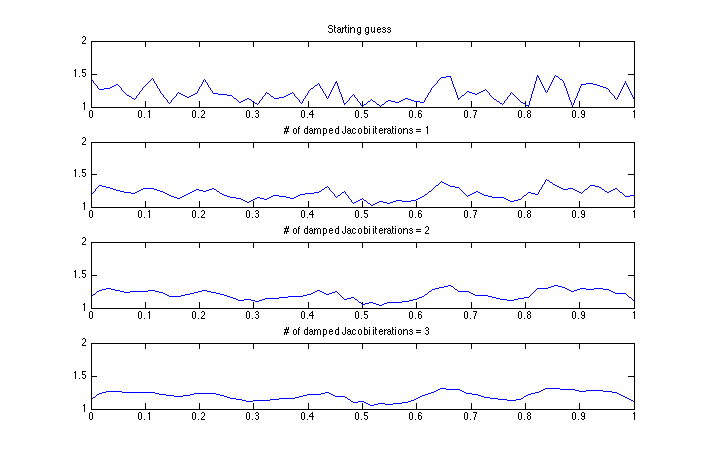
\includegraphics[width=4in]{dampedjacobi}
\caption{3 iterations of damped Jacobi}
\label{fig:dampedjacobi}
\end{figure}
From just a few iterations one can see that the residual has been effectively smoothed, though the magnitude has not been reduced that much. This is why these simple iterative methods have poor convergence properties for smooth residuals. A key idea in multigrid is that  smooth residual ($r$) then can be restricted onto a coarser grid with $m<n$ variables.

{\bf Step 2: Restriction}

By defining a restriction operator $P^{\mbox{\tiny{T}}}:\mathbb{R}^n \rightarrow \mathbb{R}^m$ we can define the smoothed residual onto the coarser grid by $r_c = P^{\mbox{\tiny{T}}}r$. On the same coarse grid we can define the coarse grid operator by $A_c = P^{\mbox{\tiny{T}}}AP$ (the new operator is called the Galerkin operator).

{\bf Step 3: Solve}

On the coarse grid we solve $A_ce_c = r_c$ for the coarse grid error $e_c$.


{\bf Step 4: Prolongation and correct}

From step 3 we solved our smaller system on a coarse mesh. We then need to prolongate the error, $e_c$, back onto the original mesh. We do this by taking our intial $x$ and adding the prolongated $e_c$ to it, i.e. $x = x+Pe_c$. Notice that the prolongation, $P$, is the transpose of the restriction operator.




What I have described above is known as a two-grid cycle (see figure~\ref{fig:TwoGrid}).
\begin{figure}[h!]
\centering
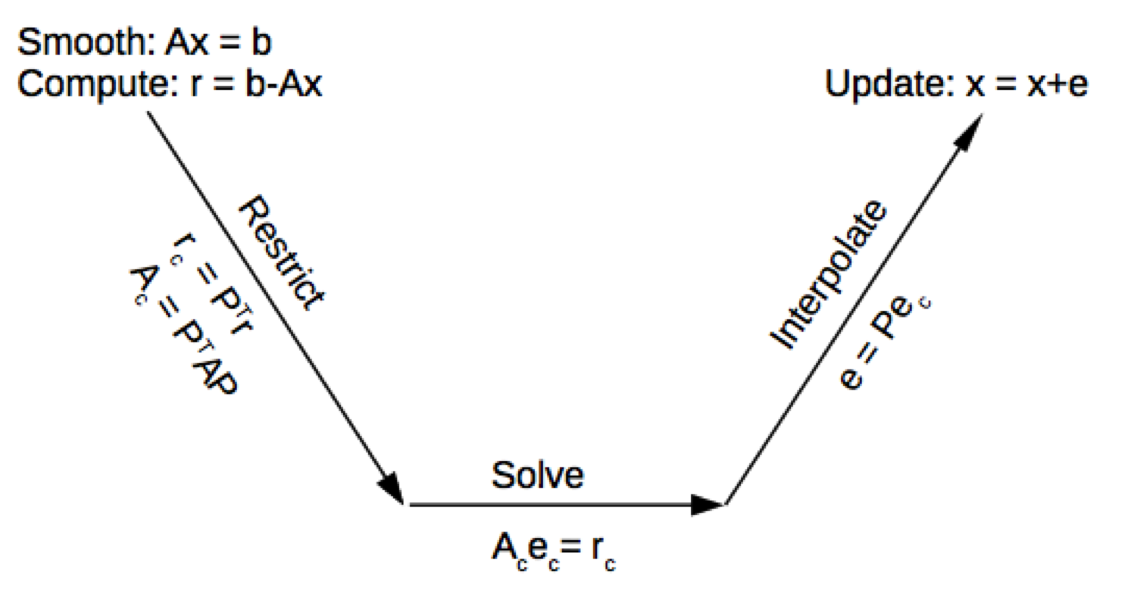
\includegraphics[width=2.5in]{../figures/TwoGrid}
\caption{Two grid cycle}
\label{fig:TwoGrid}
\end{figure}
Instead of doing a direct solve at step 2 we could apply another two-grid cycle. Therefore, this algorithm can be done recursively. One type of recursive multigrid cycle is known as a V-Cycle (see figure~\ref{fig:vcycle}). From the figure we can see that the process is fairly simple: we restrict the residual to coarser and coarser grids with different multiples of $h$ and then interpolate or prolongate back to the original grid with mesh size $h$.
\begin{figure}[h!]
\centering
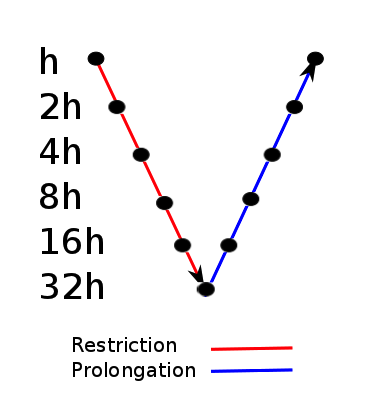
\includegraphics[width=1.5in]{Vcycle}
\caption{Multigrid V-cycle}
\label{fig:vcycle}
\end{figure}

To illustrate how effective multigrid can be and why we would like to use it, a simple $2D$ MATLAB script was written that performs a simple GMG V-cycle as a preconditioner to Conjugate Gradients (CG) for Poisson's equations. We also tested the code with an incomplete Cholesky factorisation as a preconditioner and MATLAB's inbuilt direct solve to produce the following table.
\begin{table}[h]
\centering
\caption{}
\begin{tabular}{*{7}{c}}
\hline
 Grid  &      Matrix & \multicolumn{2}{c}{MG} & \multicolumn{2}{c}{ICHOL}& Direct  \\
 Size     &     Size    &       iters       &        time       &       iters       &        time       &        time     \\
\hline
$15  ^2 $ &    225    &    5   &    0.0113   &    17    &    0.0030    &    0.0004  \\
$31  ^2 $ &    961    &    6   &    0.0096    &    30    &    0.0060    &  0.0009 \\
$63  ^2 $ &    3969    &    6   &    0.0193    &    55    &    0.0223    &    0.0042 \\
$127 ^2$   &    16129    &    6   &    0.0470    &    102    &    0.1103    &    0.0185  \\
$255 ^2$   &    65025    &    6   &    0.1602    &    187    &     0.7753    &    0.0914  \\
$511 ^2$   &    261121    &    6   &    0.6182    &    339    &    5.473    &    0.4888  \\
$1023^2$    &    1046529    &    6   &    2.6700   &   576    &   38.4429    &    2.2417   \\
$2047^2$    &    4190209    &    6    &    11.1644    &    1021    &    279.704    & 11.6493  \\
$4095^2$      &      16769025     &      6      &    47.1795    &     2001    &    2478.998    &    -  \\

\hline
\end{tabular}
\caption{Timing and iteration results for the Poisson problem using GMG}
\label{tab:multitest}
\end{table}
The - in the table means that we ran out of memory. Table~\ref{tab:multitest} shows that as we increase the mesh size then the number of iterations of CG when using a multigrid V-cycle stays constant. This is the attraction of using a multigrid method. The constant number of iterations we see when using a multigrid V-cycle is not apparent when we use an incomplete Cholesky factorisation. Indeed we see that as the size of the mesh increases the number of iterations roughly doubles. This shows the scalability power of GMG.

\section{Algebraic Multigrid} \label{sec:AMG}

In the previous section we looked at how a GMG scheme worked. One of the main principles of GMG is that we have a sequence of grids (usually uniform grids) on which we can define interpolation and restriction operators. However, if you are considering a discretisation on an unstructured grid then it is very hard (usually impossible) to produce interpolation and restriction operators which would map the fine unstructured grid to a coarse unstructured grid. Therefore, we would like to be able to construct interpolation and restriction operators based solely on the coefficients of the matrix. This leads to an algebraic multigrid (AMG) approach.

% The general structure of AMG is the same as for GMG (breif description given above). However, in GMG the next levels grid defines the interpolation and restriction operators but AMG relies on just the coefficients of the matrix to define the operators.

In the rest of this section we will go through the process of forming these interpolation and restriction operators for the classical AMG (CAMG) following \cite{brandt1985algebraic,ruge1987algebraic,brandt1986algebraic}.

\subsubsection*{Smoothness}

CAMG is established on the presumption that geometrically smooth functions are in the near null space of $A$. As we have no geometric information to use we need to find an algebraic way to define smoothness. Defining $(\lambda,e)$ to be the eigenvalue-eigenvector pairs for a symmetric $A$, then smoothness is characterised as
\begin{equation} \label{eq:smoothness}
    e^{\mbox{\tiny{T}}}Ae = \lambda \ll 1.
\end{equation}
To make things a little easier we assume that $A$ has been normalised (to ensure that $\lambda_{\mbox{\tiny{max}}}=1$). From our assumption (geometrically smooth functions are in the near null space) and the further assumption that the row sums of A are zero then we can rearrange (\ref{eq:smoothness}) to be
\begin{equation} \label{eq:smooth}
    \begin{aligned}
        e^{\mbox{\tiny{T}}}Ae &= \sum_i e_i\big( a_{ii}e_i\sum_{i\neq j} a_{ij}e_i\big),\\
                                               &= \sum_i e_i\big( \sum_{i\neq j} (-a_{ij})(e_i-e_j)\big),\\
                                               &= \sum_{i<j} (-a_{ij})(e_i-e_j)^2 \ll 1.
    \end{aligned}
\end{equation}
From (\ref{eq:smooth}) we can see that smooth error changes slowly for large matrix coefficients. This leads to one of the main concepts within AMG: Strength of Connection.
\begin{mydef} \label{def:SOC}
Strength of Connection:

Given $\theta \in (0,1]$, variable (point) $u_i$  strongly depends on the variable (point) $u_j$ if
$$-a_{ij}\geq \theta \max_{k\neq i} \{-a_{ik}\}.$$

\end{mydef}

From \textbf{Definition \ref{def:SOC}}, strength of connection is measured corresponding to the largest off-diagonal entry in each row.


\subsubsection*{Coarse "grid" selection}

In CAMG, the set of coarse points (C-points) are a subset of the fine points (F-points). The C-points are chosen in the direction of strong connections of the matrix. To define the coarse grid we do the following three steps:
\begin{itemize}
  \item[1.] Define strength matrix $A_s$ using \textbf{Definition  \ref{def:SOC}}
  \item[2.] \textbf{Phase 1:} Choose set of fine points based on $A_s$
  \item[3.] \textbf{Phase 2:} Choose extra points to satisfy interpolation requirements
\end{itemize}
The easiest way to show this procedure is to look at a simple example. The example we will look at is a finite element discretisation of the 2D Laplacian matrix with the following 9-point stencil:
\begin{equation} \label{eq:stencil}
 \begin{pmatrix}
     -1 &-1&-1\\
     -1 &8&-1\\
     -1 &-1&-1
   \end{pmatrix}.
\end{equation}
This is in fact a discretisation stencil on a uniform grid but the grid selection will not use any geometric information. From the stencil (\ref{eq:stencil}) we note that all the off-diagonal entries of the matrix will be $-1$'s. Hence, the strength matrix $A_s$ will be exactly the same as the original matrix $A$.

The degree of a node is defined by how many neighbouring nodes depend upon it. Figure \ref{fig:1to3} to \ref{fig:7to9} show the degree of the node at the $(i,j)$ point on the grid. This therefore means that we don't use any geometric information to form these coarse grids.

\textbf{Phase 1:} Choose set of C and F-points
\begin{itemize}
    \item[i. ] From strength matrix $A_s$ select a C-point with maximal measure (Figure \ref{fig:1to3}(b))
    \item[ii. ] Set the neighbours of the C-point to be F-points (Figure \ref{fig:1to3}(c))
    \item[iii. ] Update the F-point neighbours so that they are more likely to be chosen  (Figure \ref{fig:4to6}(a))
    \item[iv. ] Repeat steps i. to iii. (Figure \ref{fig:4to6} and \ref{fig:7to9})
\end{itemize}

\begin{figure}[h!]
\begin{center}$
\begin{array}{ccc}
\subfigure[Step 1]{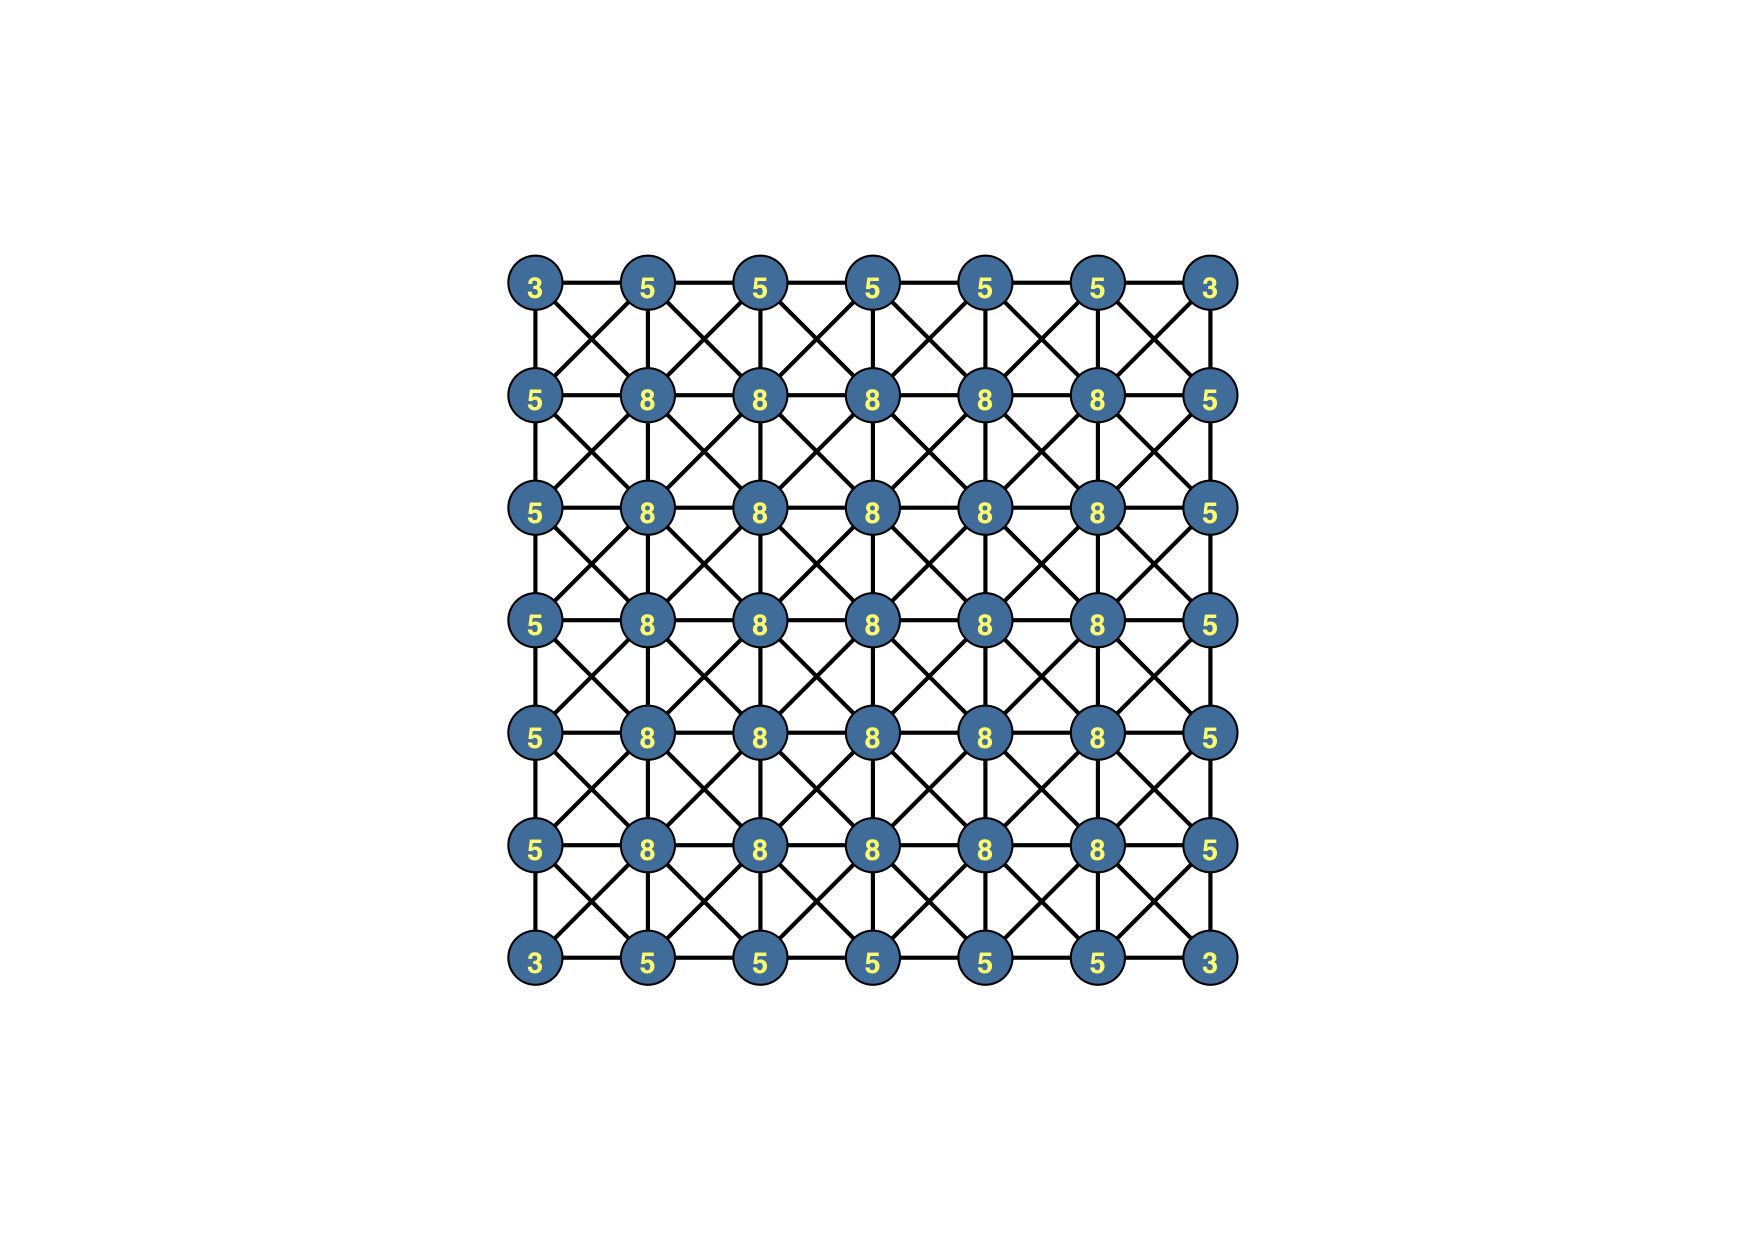
\includegraphics[trim = 85mm 40mm 85mm  40mm, clip, width=1.5in]{figures/AMG1.png} }&
\subfigure[Step 2]{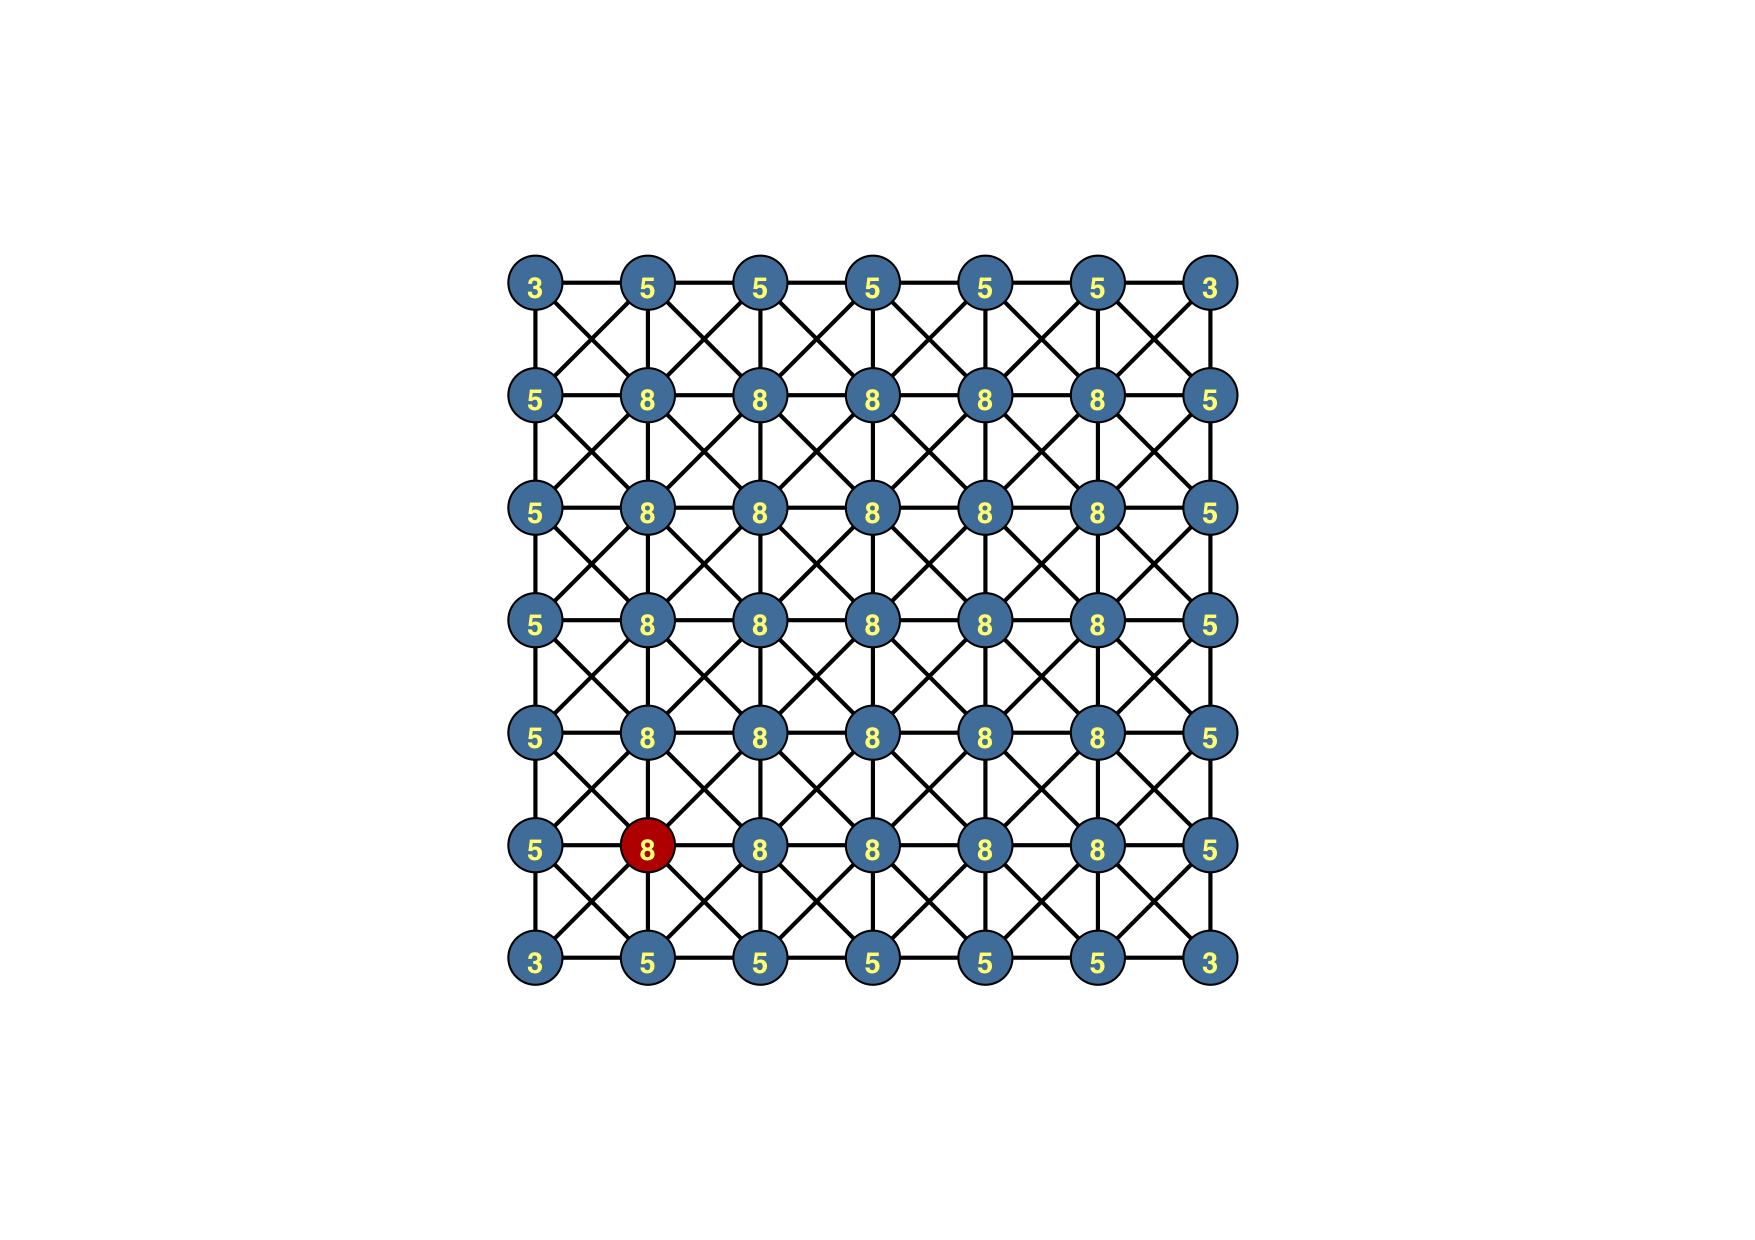
\includegraphics[trim =   85mm 40mm   85mm  40mm, clip, width=1.5in]{figures/AMG2.png}} &
\subfigure[Step 3]{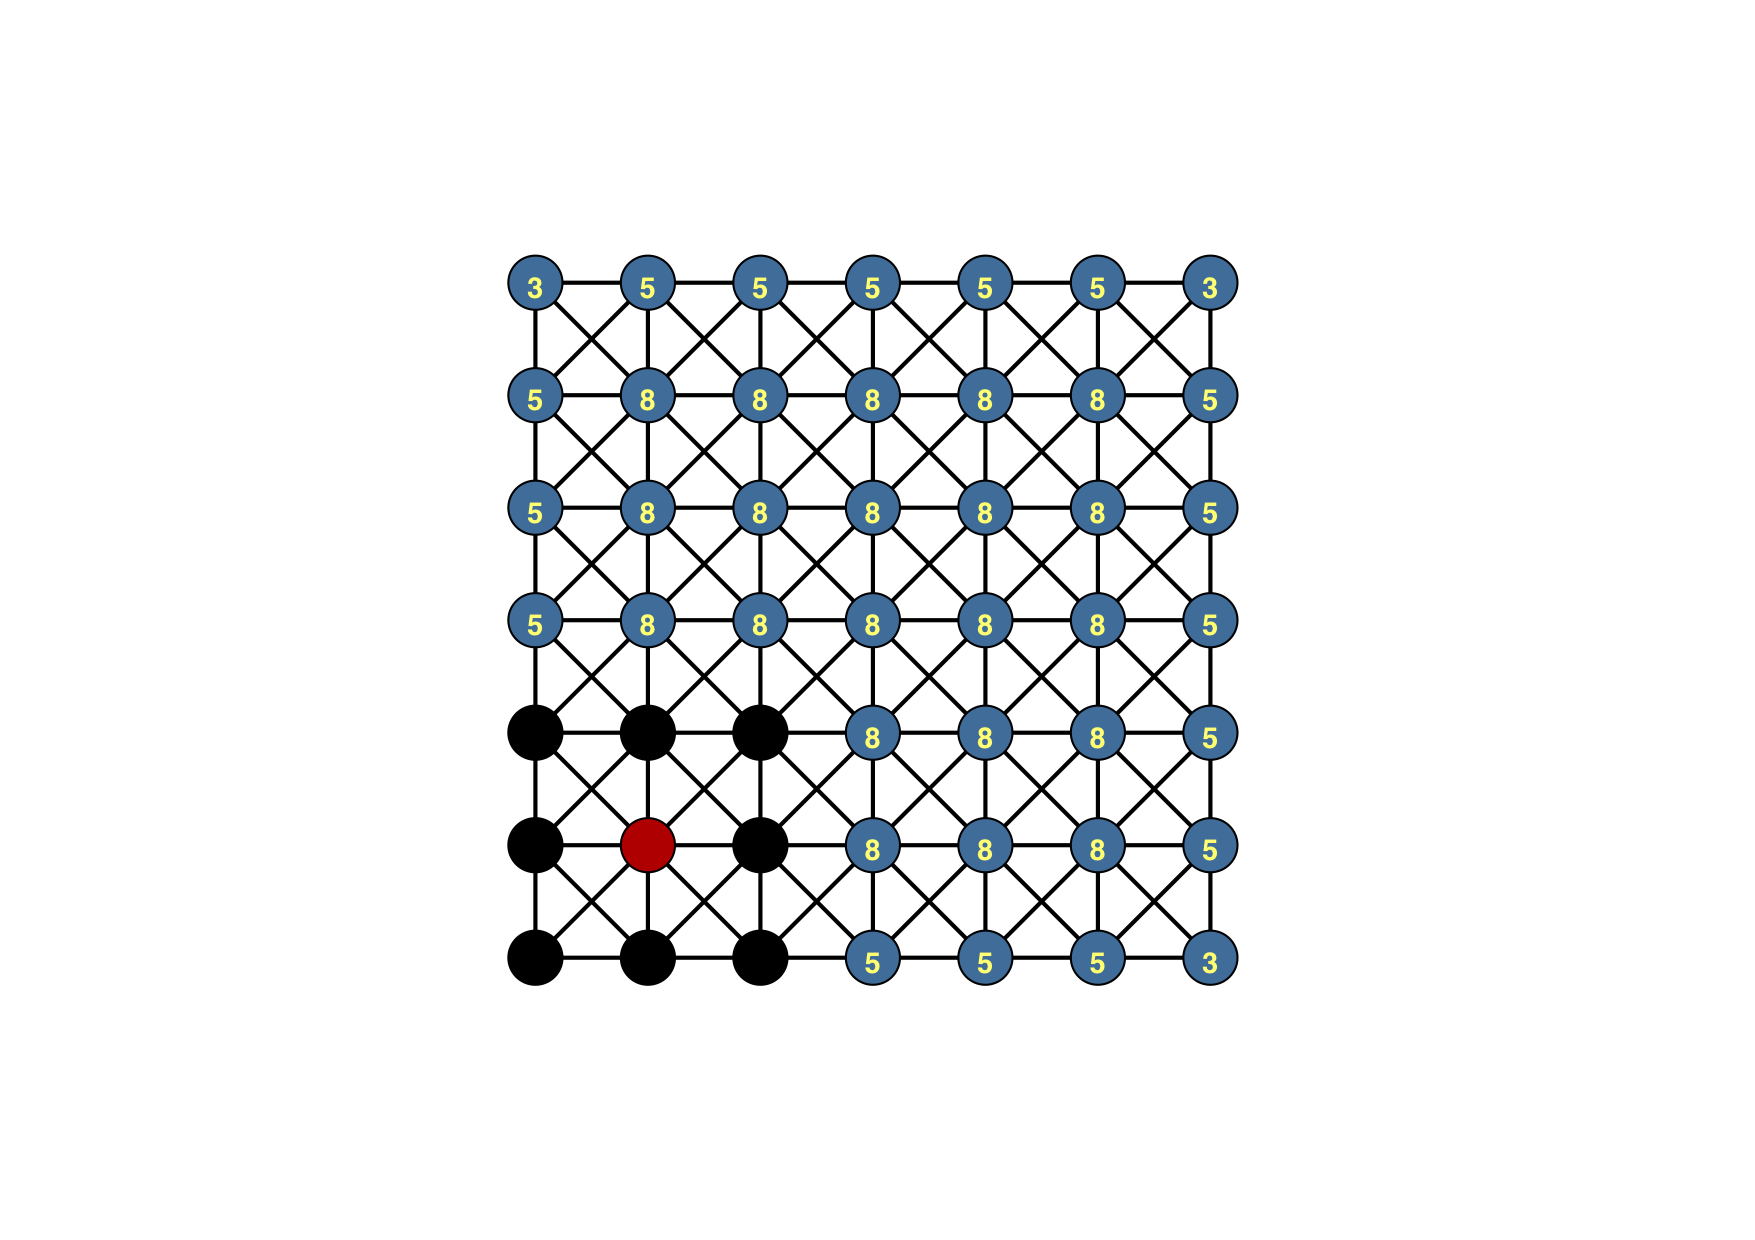
\includegraphics[trim =   85mm 40mm   85mm  40mm, clip, width=1.5in]{figures/AMG3.png}}
\end{array}$
\caption{Steps 1 to 3 from \cite{falgout2006introduction}}
\label{fig:1to3}
\end{center}
\end{figure}

\begin{figure}[h!]
\begin{center}$
\begin{array}{ccc}
\subfigure[Step 4]{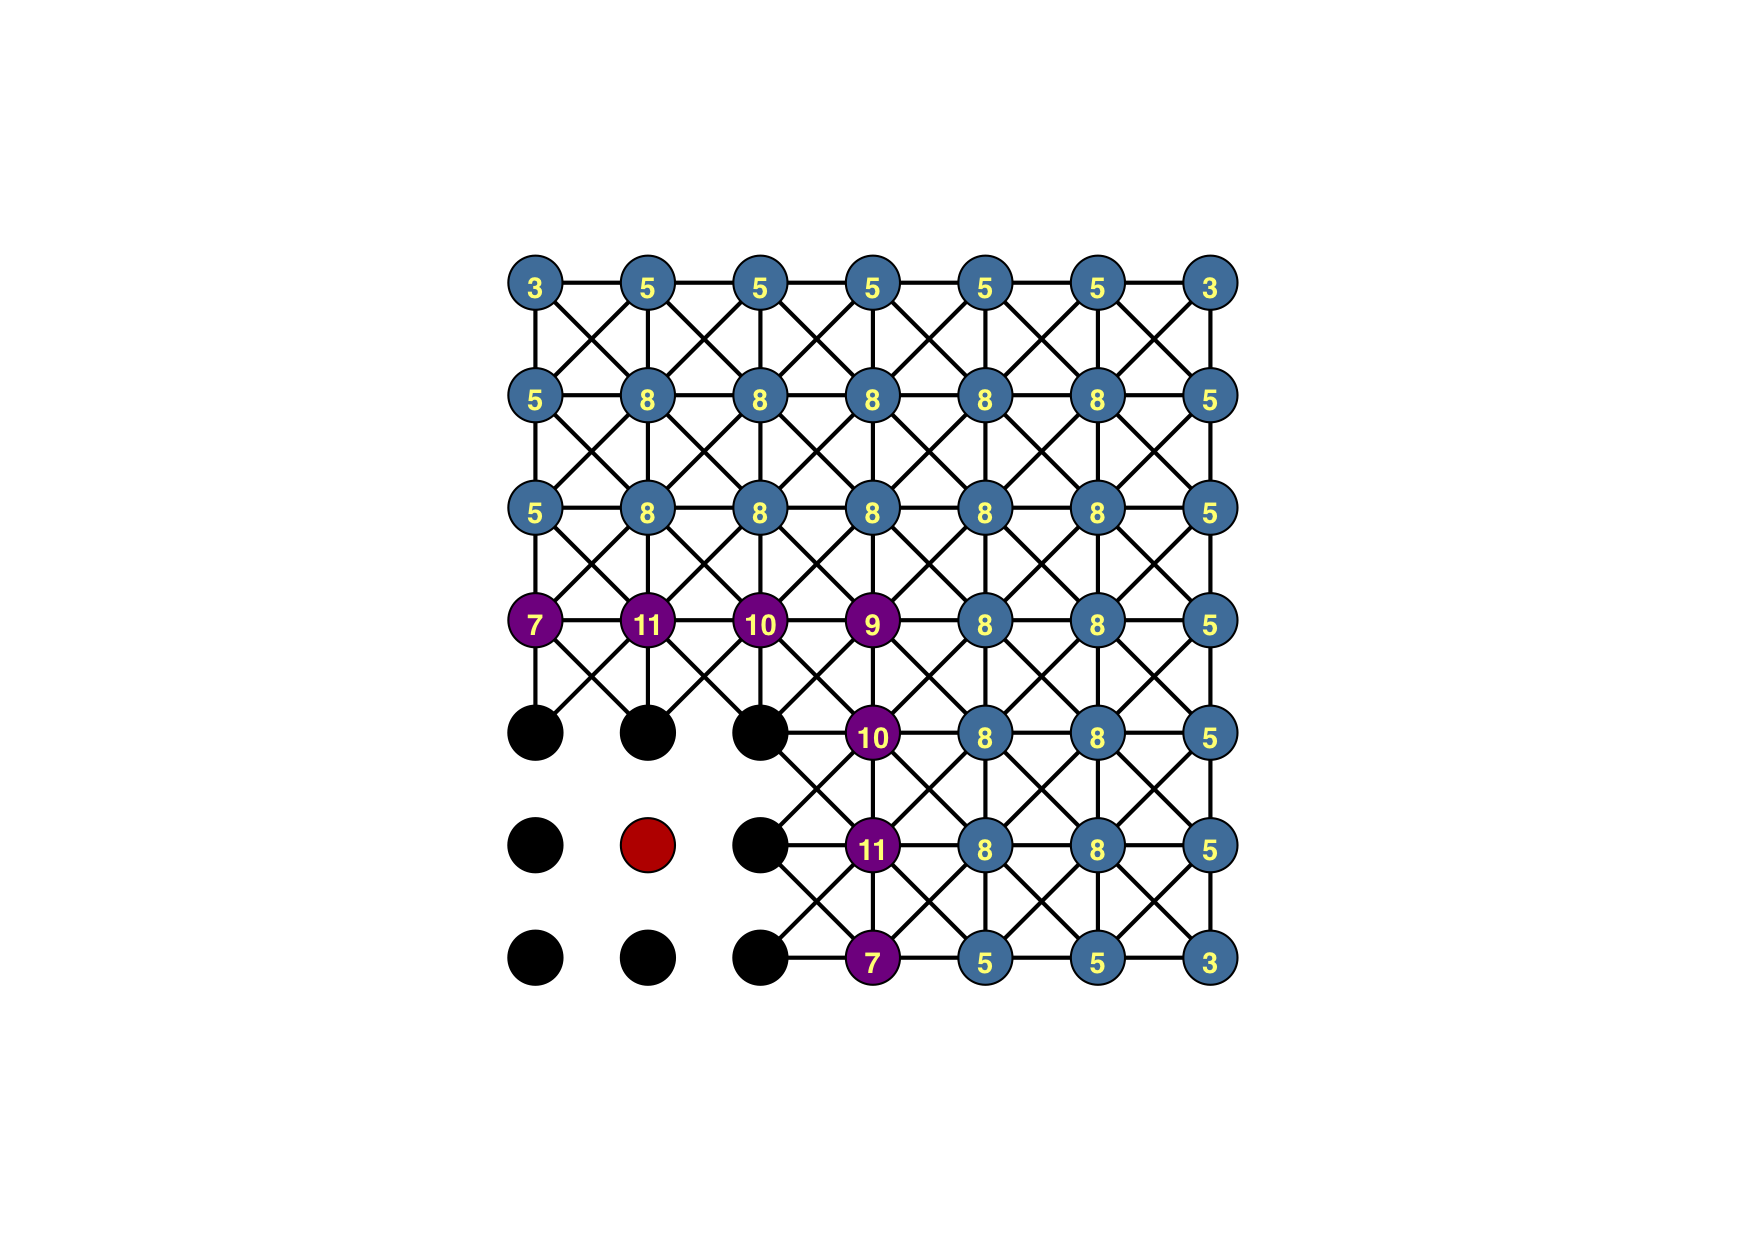
\includegraphics[trim = 85mm 40mm 85mm  40mm, clip, width=1.5in]{figures/AMG4.png} }&
\subfigure[Step 5]{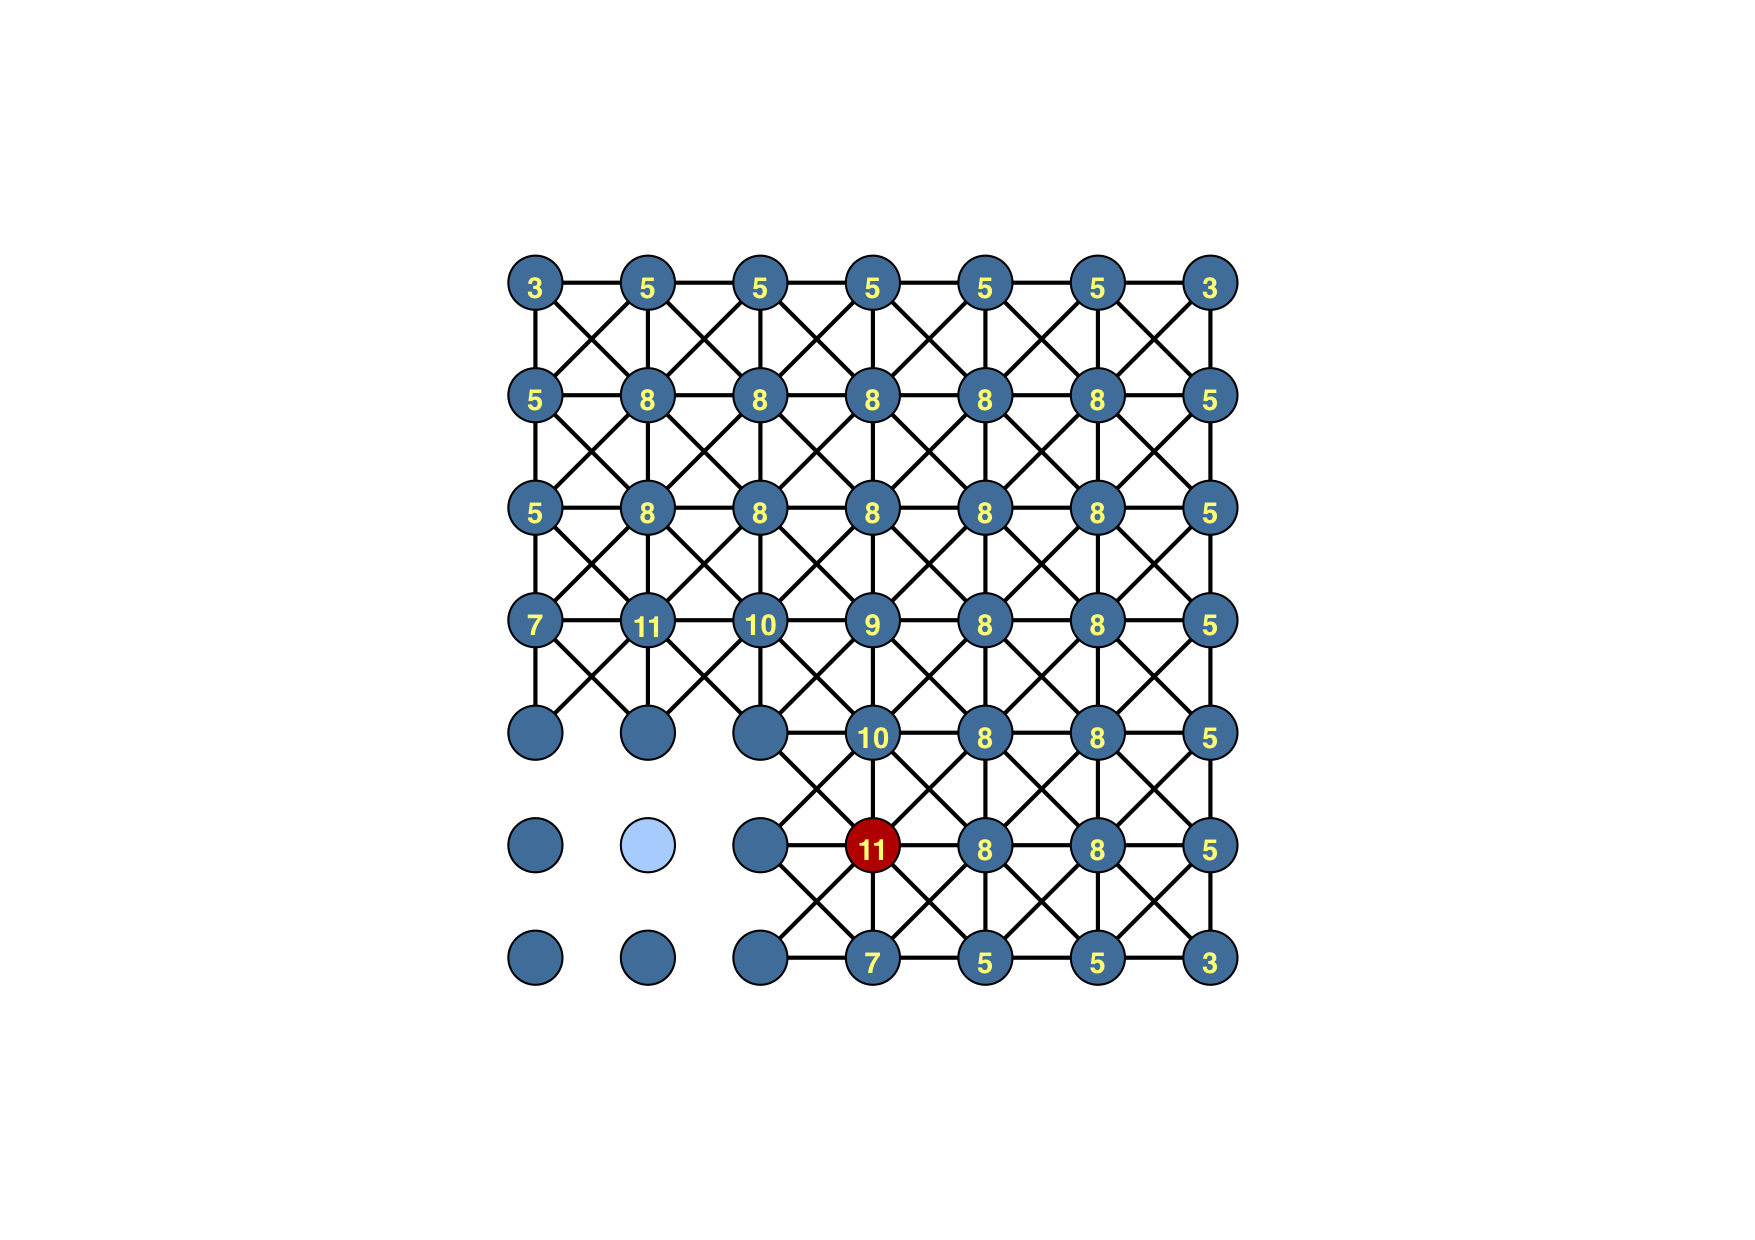
\includegraphics[trim =   85mm 40mm   85mm  40mm, clip, width=1.5in]{figures/AMG5.png}} &
\subfigure[Step 6]{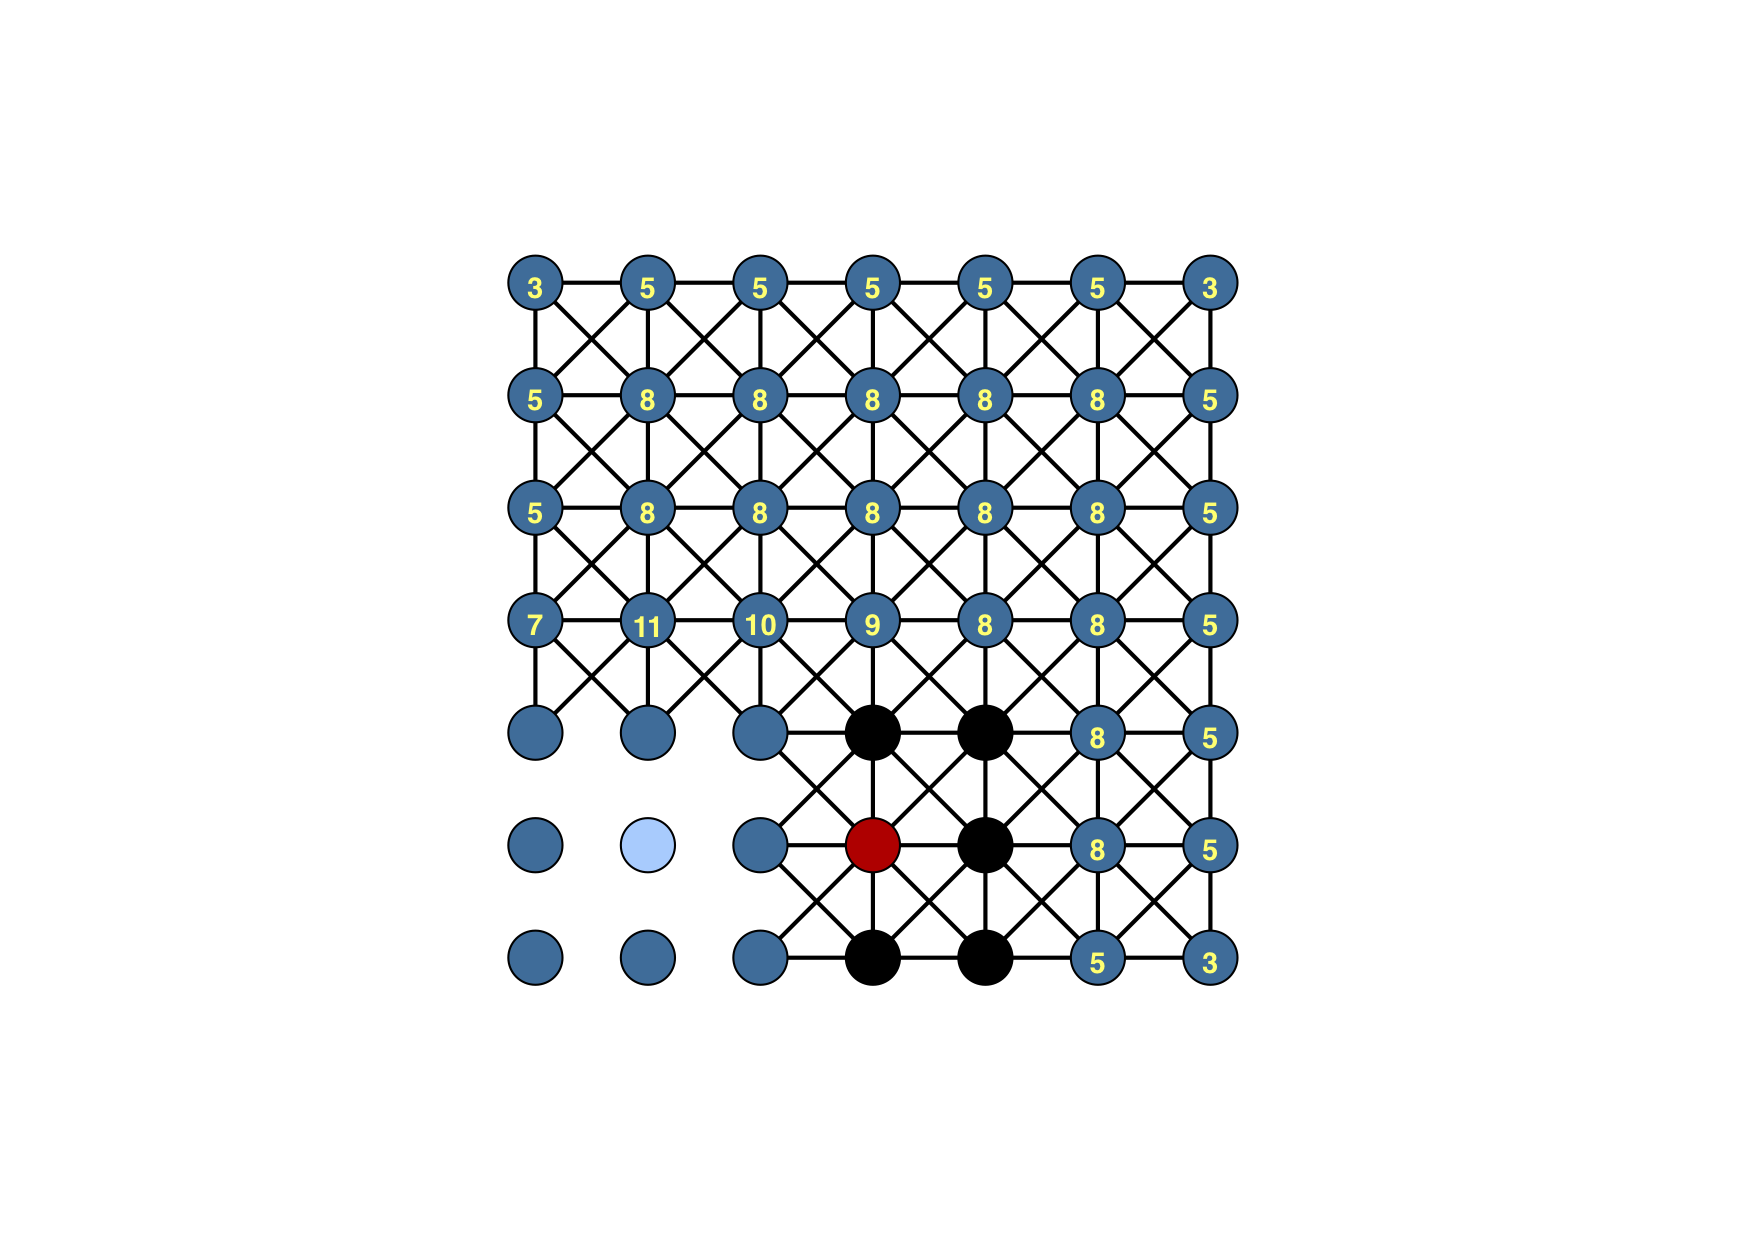
\includegraphics[trim =   85mm 40mm   85mm  40mm, clip, width=1.5in]{figures/AMG6.png}}
\end{array}$
\caption{Steps 4 to 6 from \cite{falgout2006introduction}}
\label{fig:4to6}
\end{center}
\end{figure}

\begin{figure}[h!]
\begin{center}$
\begin{array}{ccc}
\subfigure[Step 7]{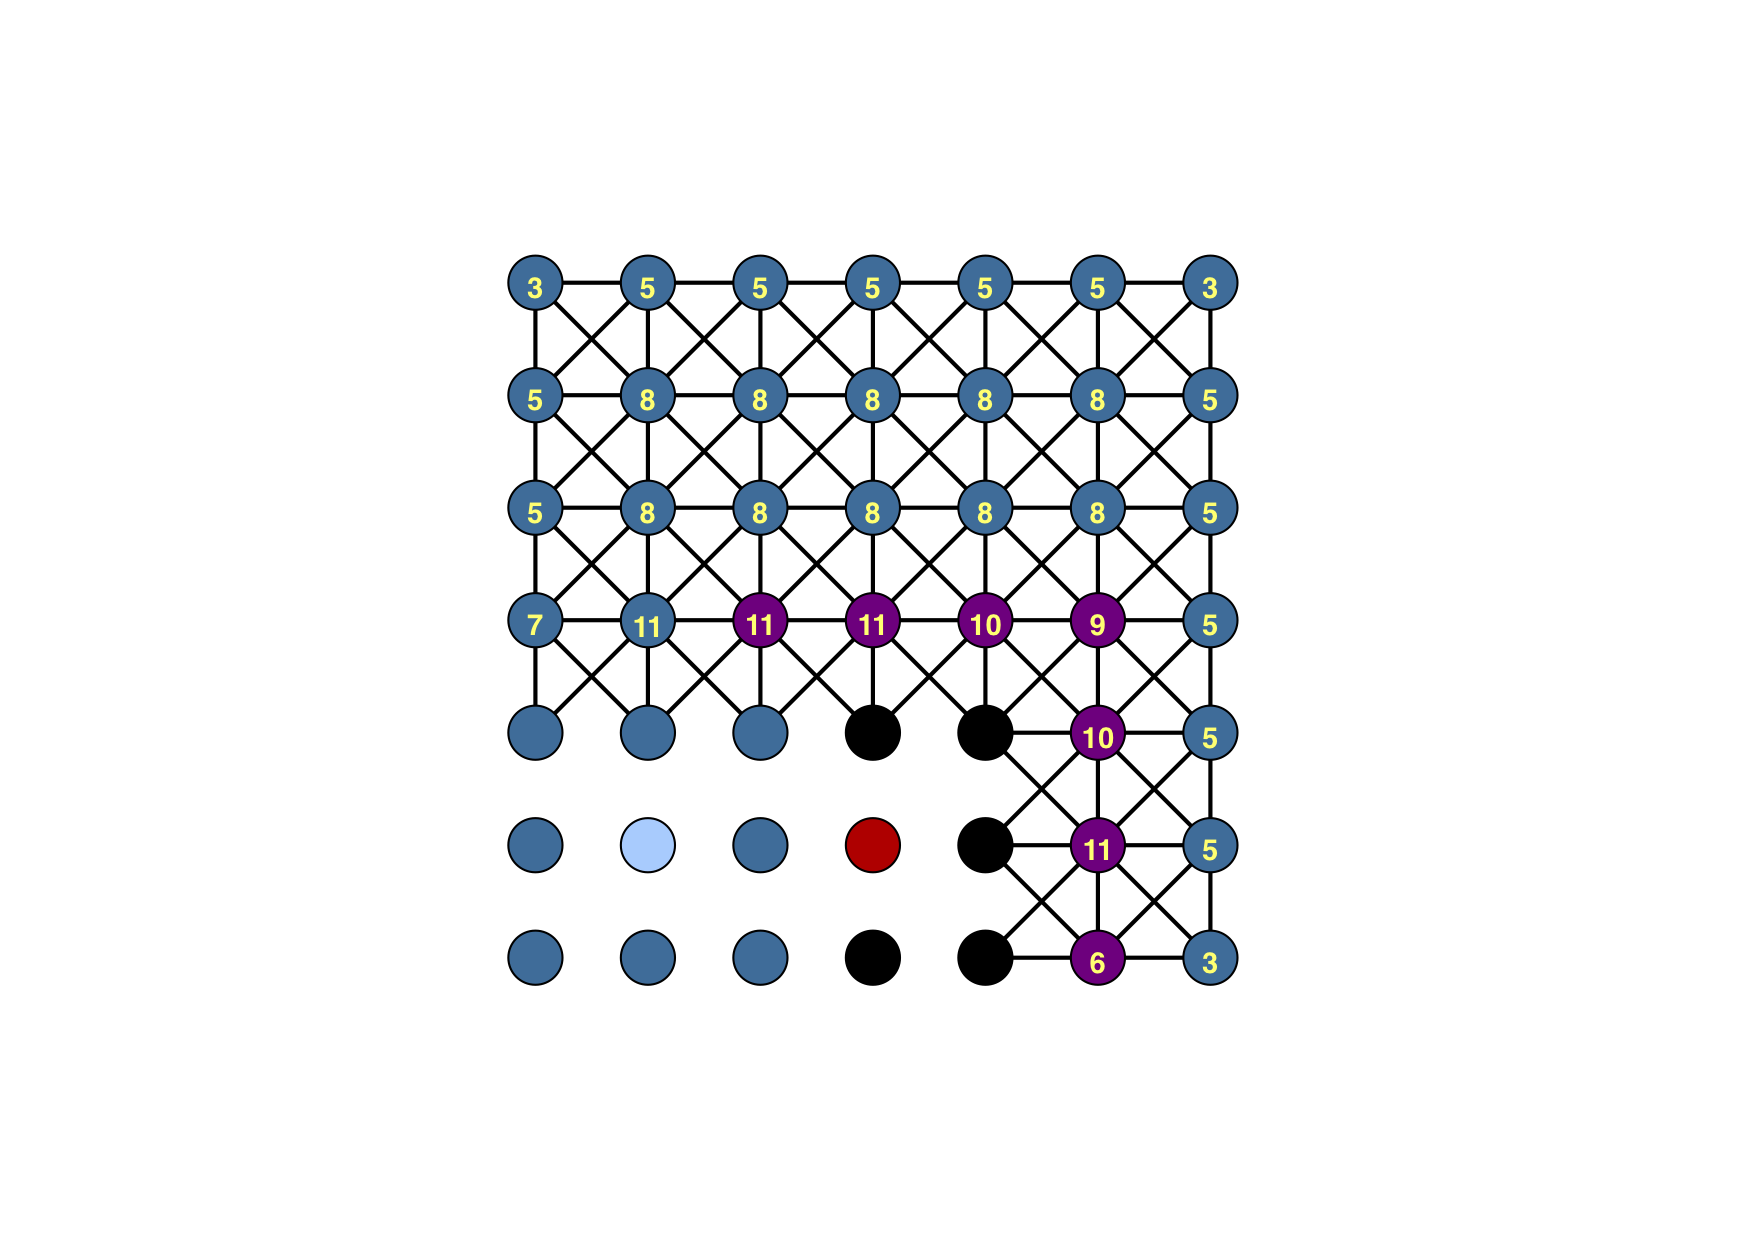
\includegraphics[trim = 85mm 40mm 85mm  40mm, clip, width=1.5in]{figures/AMG7.png} }&
\subfigure[Step 8]{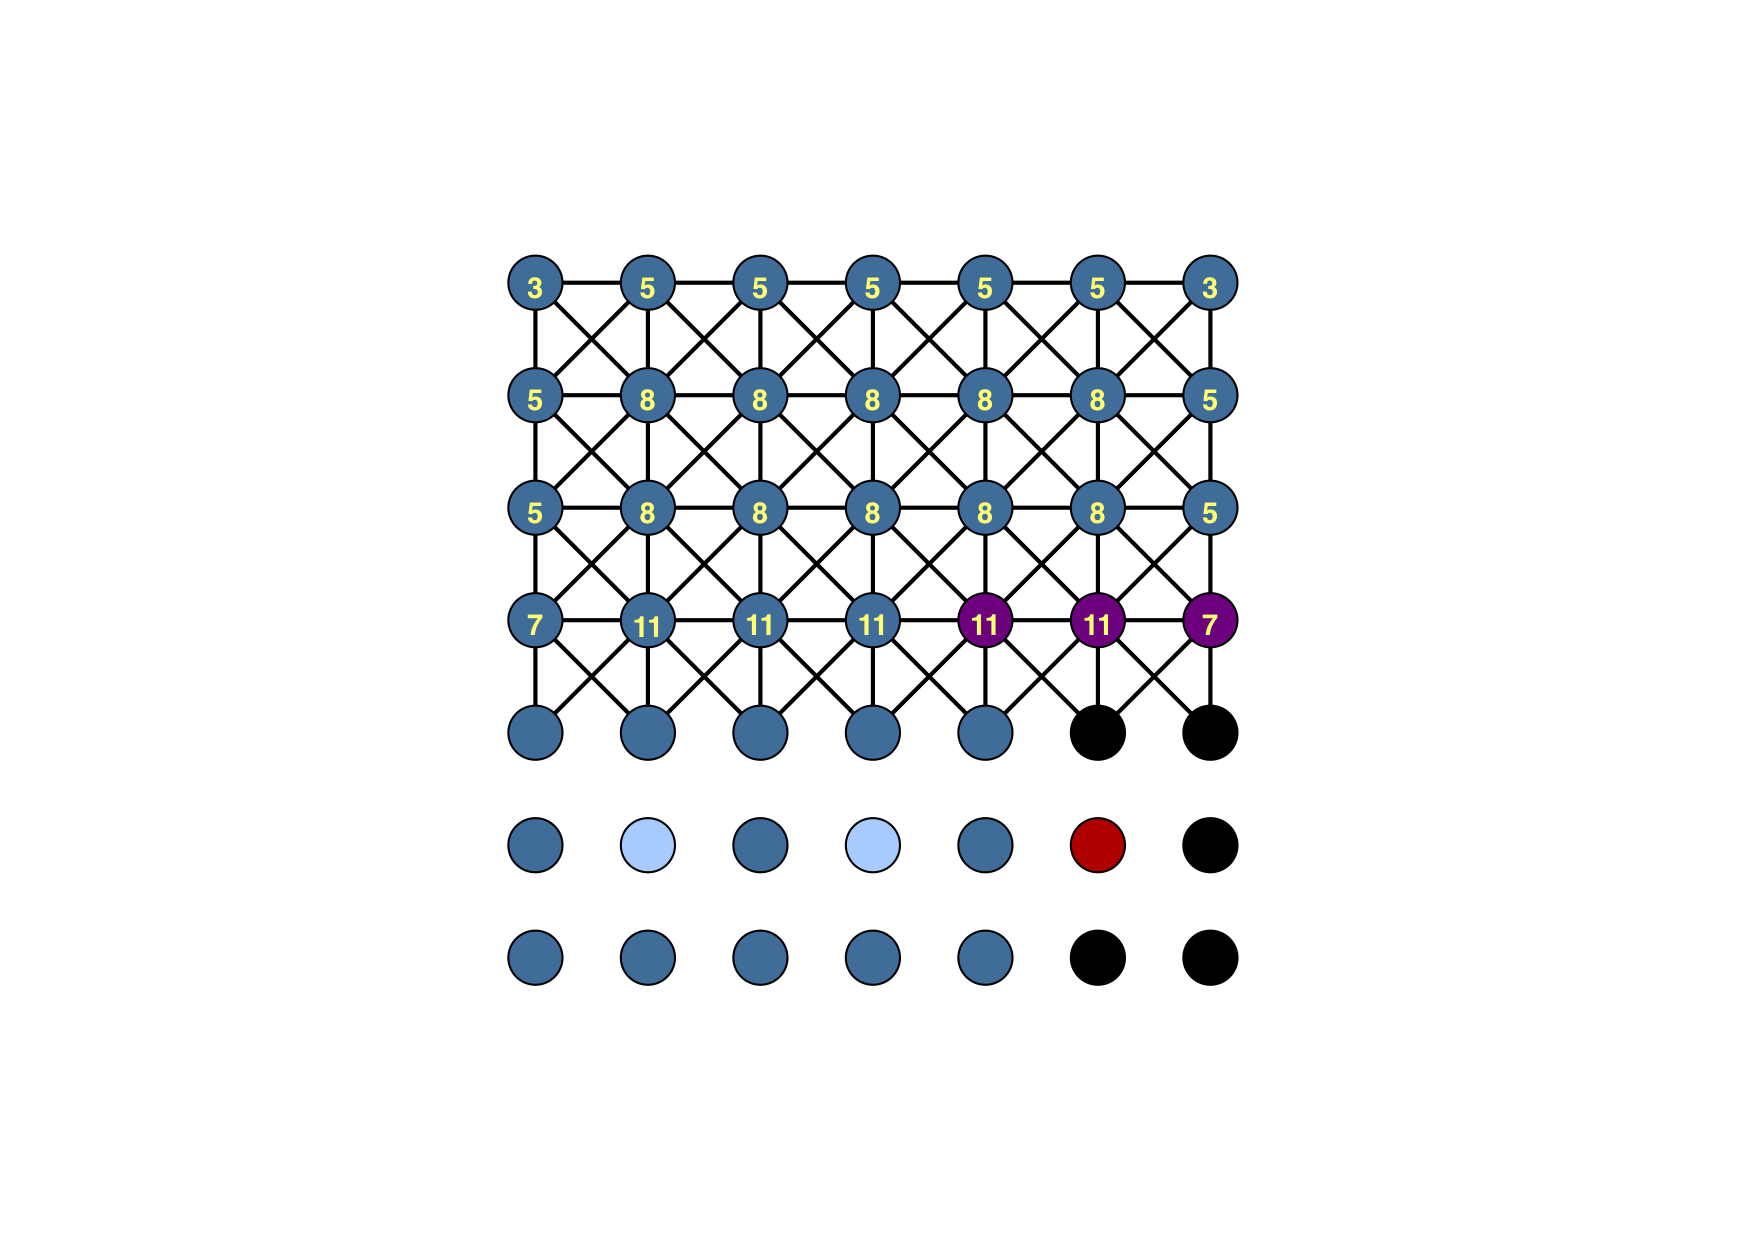
\includegraphics[trim =   85mm 40mm   85mm  40mm, clip, width=1.5in]{figures/AMG8.png}} &
\subfigure[Step 9]{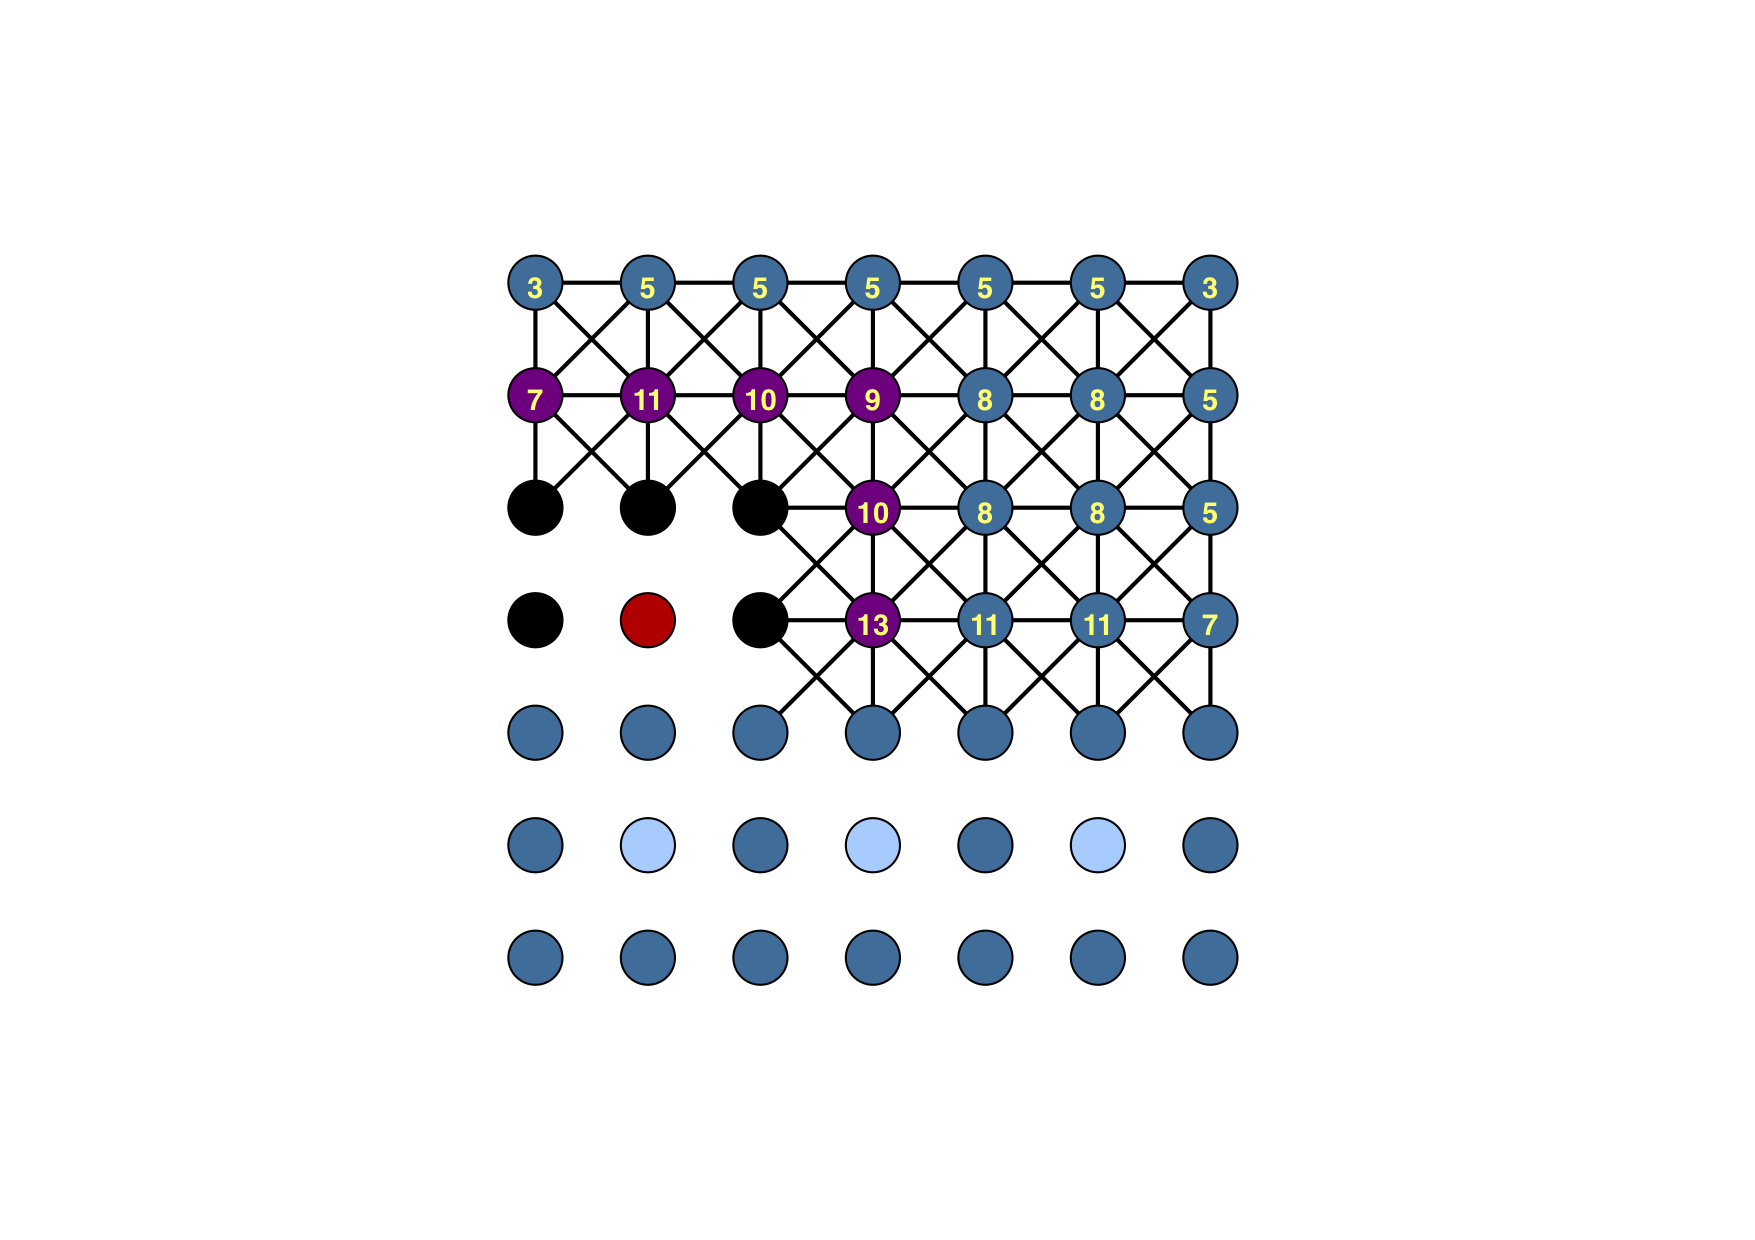
\includegraphics[trim =   85mm 40mm   85mm  40mm, clip, width=1.5in]{figures/AMG9.png}}
\end{array}$
\caption{Steps 7 to 9 from \cite{falgout2006introduction}}
\label{fig:7to9}
\end{center}
\end{figure}


Carrying out this sequential process yields the coarsened grid given in figure \ref{fig:coarsegride}.
\begin{figure}[h!]
\begin{center}
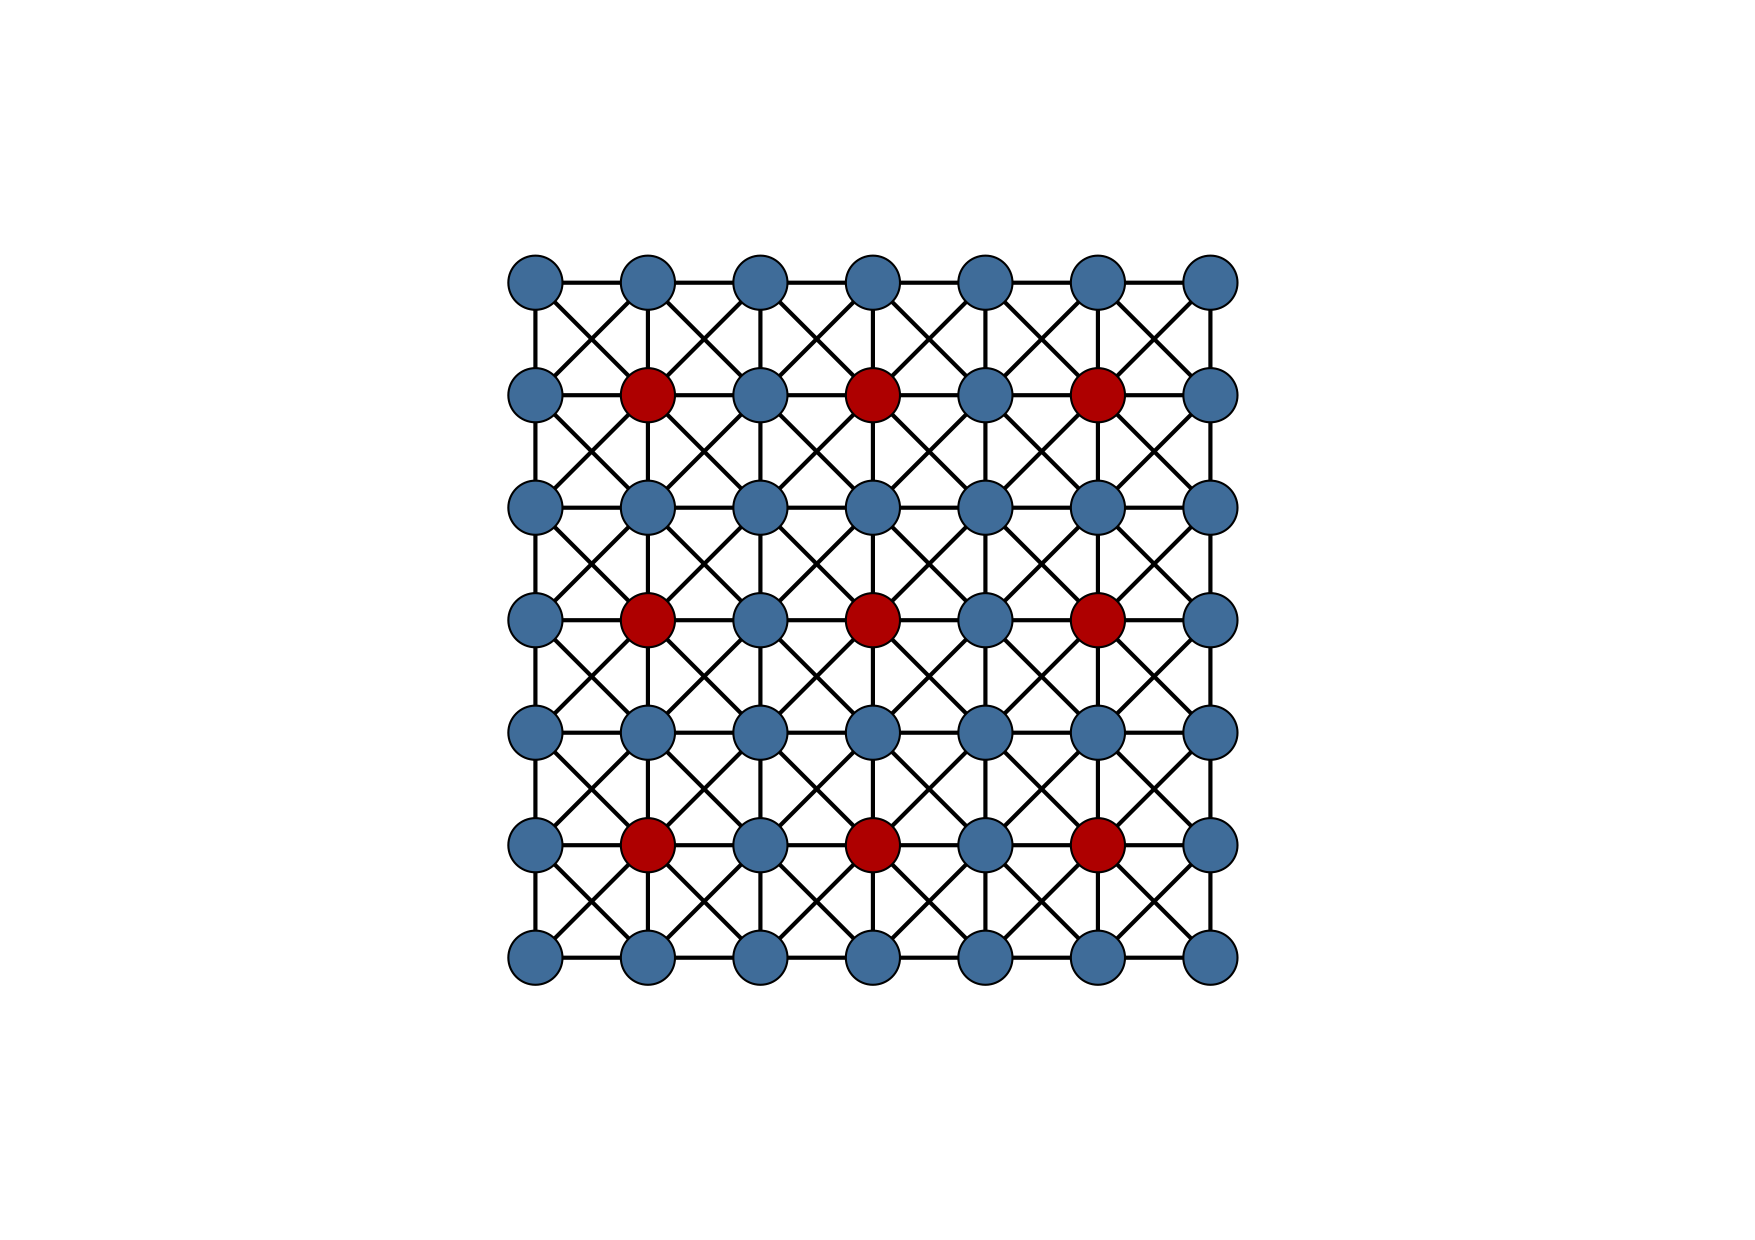
\includegraphics[trim = 85mm 40mm 85mm  40mm, clip, width=2in]{../figures/AMG10.png}
\caption{C-point (red) and F-points (blueish) from \cite{falgout2006introduction}}
\label{fig:coarsegride}
\end{center}
\end{figure}

\textbf{Phase 2:} Satisfy interpolation requirements

CAMG requires that all strongly connected F-point pairs must be strongly connected to a common C-point. Therefore, we loop through the F-points to find strongly connected pairs. If we find strongly connected pairs then we check if they are strongly connected to a common C-point. If they are then we move onto the next F-point pair, otherwise we make one of the F-points a C-point.

This second phase leads to higher complexity within the algorithm so more recent AMG methods don't do this and modify interpolation instead.


\subsubsection*{Interpolation}

Recall that we defined algebraic smoothness by (\ref{eq:smoothness}). Since the residual can be defined as $r = Ae$, then re-writing (\ref{eq:smoothness}) gives us:
$$\lambda^2 = e^{\mbox{\tiny T}} A^2e = r^{\mbox{\tiny T}}r = ||r|| \ll1.$$
This shows that we can characterise smoothness by a small residual. CAMG uses this property to define interpolation operators. CAMG sets the residual to be point wise $0$ i.e.
$$r_i = (Ae)_i = 0.$$
Re-write this equation in terms of $3$ separate sets gives
\begin{equation}\label{eq:3separate}
    a_{ii}e_i = -\sum_{j\in C_i} a_{ij}e_j -\sum_{j\in F_i} a_{ij} e_j -\sum_{j\in N_i} a_{ij}e_j
\end{equation}

\hspace{.25in}$C_i$: C-points strongly connected to $ i$

\hspace{.25in}$F_i$: F-points strongly connected to $i$

\hspace{.25in}$N_i$: all points weakly connected to $i$

\noindent Define $C_i$ as the set of interpolatory points. Then the goal is to express these points in terms of the points in the sets of $F_i$ and $N_i$.  Returning to the 2D FE Laplacian example then $N_i$ is simply just the empty set. Therefore the aim is to come up with an interpolation that maps the C-Points to the F-points. This is called collapsing the stencil. Again, we will be doing this in a pictorial way as it is easier to visualise (Figure \ref{fig:stencil}).
\begin{figure}[h!]
\begin{center}
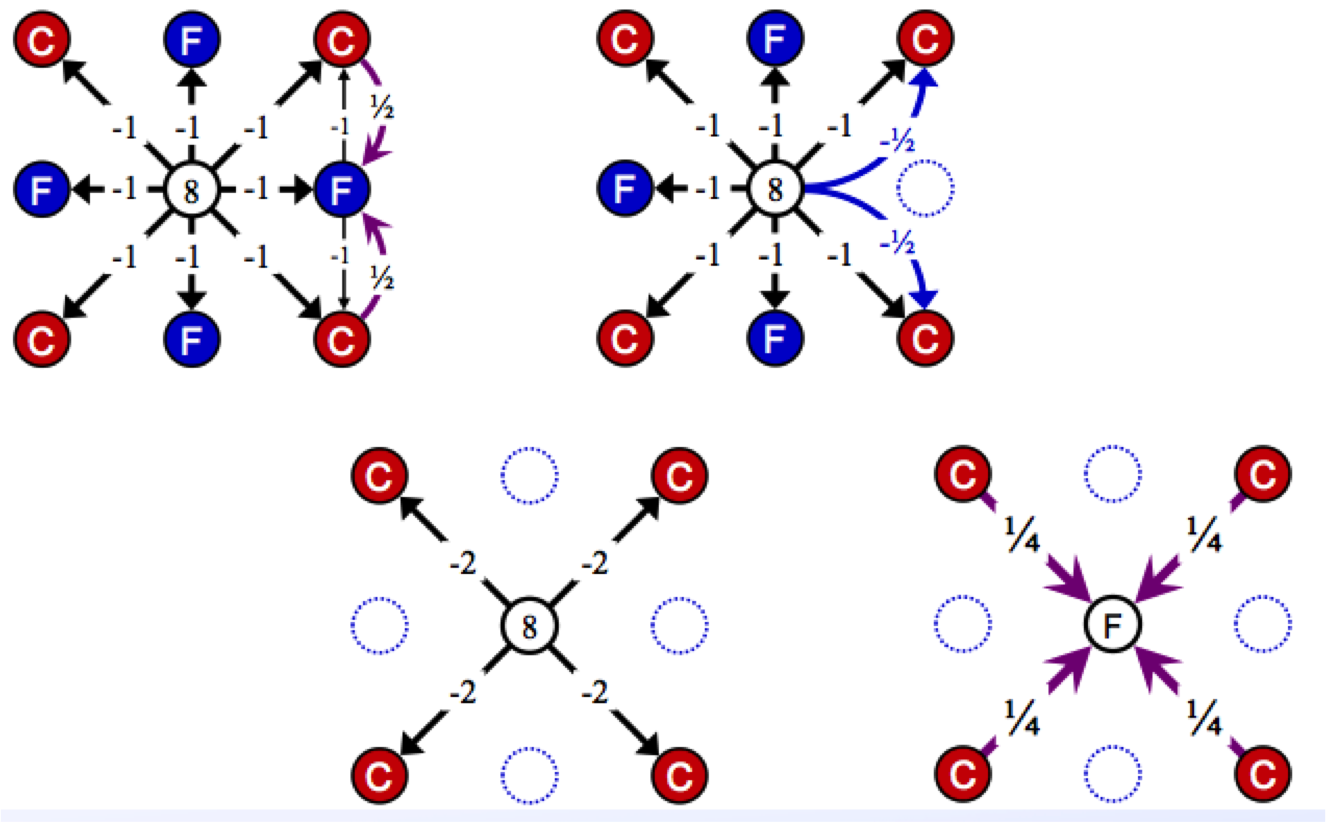
\includegraphics[width=4.2in]{../figures/Interp.png}
\caption{Collapsing the stencil from \cite{falgout2006introduction}}
\label{fig:stencil}
\end{center}
\end{figure}


After one has produced the interpolation stencil we have all the ingredients needed for multigrid. We simply define $P^{\mbox{\tiny T}}$ from the coarse set of variables and apply either a two-grid cycle or V-cycle depending the problem.

The method that we have gone through here is the classical Ruge-St{\"u}ben AMG. However, there are many variations on this method that could suit a particular problem better. The other main class of AMG is known as smoothed aggregation AMG. This method follows the same structure as CAMG but forms aggregates when forming the coarse grids. This generally leads to coarse grids with smaller dimension for each level of the multigrid V-cycle.


\section{Stokes Equations} \label{sec:stokes}


 To illustrate how effective AMG can be, we look at Stokes equations given in (\ref{eq:Stokes})
\begin{equation} \label{eq:Stokes}
    \begin{aligned}
        -\nu \Delta \U+ \nabla p &= \Fs,\\
        \div \U     &= 0.
    \end{aligned}
\end{equation}
Here we define $\U$, $p$ and $\nu$ as the velocity vector, pressure and dynamic viscosity of the fluid respectively. At the moment we will not be applying AMG as a solver to this system but instead we will be applying a V-cycle as the preconditioner.

\subsection{Finite element discretisation} \label{sec:discretisation}

A weak formulation of the Stokes system (\ref{eq:Stokes}) is given by
\begin{equation} \label{eq:WStokes}
    \begin{aligned}
       \int_{\Omega}\V \cdot \big(-\nu \Delta \U+ \nabla p\big) &= \int_{\Omega} \V \cdot \Fs,\\
        \int_{\Omega} q\div \U     &= 0.
    \end{aligned}
\end{equation}
where $\V$ and $q$ are test functions choosen from a particular function space. By using vector identities and integration by parts (\ref{eq:WStokes}) can be simplified to
\begin{equation} \label{eq:WeakStokes}
    \begin{aligned}
       \int_{\Omega}\nu \nabla  \V : \nabla  \U- p \div \V &= \int_{\Omega} \V \cdot \Fs + \int_{\partial \Omega} \vec g \cdot \V,\\
        \int_{\Omega} q\div \U     &= 0.
    \end{aligned}
\end{equation}
For the test problem we will be considering purely Dirichlet boundary conditions, hence, $\vec g = 0$. Also, the notation $\nabla  \V : \nabla  \U$ represents the componentwise scalar product. For this example we will consider using Taylor-Hood elements: the function spaces are
\begin{equation} \label{eq:Spaces}
    \begin{aligned}
      \mathcal{V} =& \{\V \in H_1^2 (\Omega): \V = \vec v_0 \mbox{ on } \partial \Omega  \},\\
      \mathcal{Q} =& \{q\in H_1 (\Omega)\},
    \end{aligned}
\end{equation}
where $\U,\V \in \mathcal{V}$, $p,q\in \mathcal{Q}$ and $\vec v_0 $ is the Dirichlet boundary condition. For Stokes it is not necessary to use $q\in H_1$ as $q\in L_2$ forms a stable discretisation, however, when using Taylor-Hood elements we do in fact use $q\in H_1$. Discretisation  of (\ref{eq:WeakStokes}) using the subspaces of function spaces (\ref{eq:Spaces}) yields the following saddle point system
\begin{equation} \label{eq:system}
    \mathcal{A}x = \begin{bmatrix}
    A & B^{\mbox{\tiny{T}}}\\
    B & 0\\
    \end{bmatrix}
    \begin{bmatrix}
    u \\
    p \\
    \end{bmatrix} =
    \begin{bmatrix}
    f\\
    0 \\
    \end{bmatrix}=b.
\end{equation}

\subsection{Preconditioning} \label{sec:precond}

In this section we will  consider preconditioning Stokes equations. When applying a preconditioner to a linear system, $\mathcal{A} x = b$, we need to bear in mind the following two conditions:
\begin{itemize}
    \item[1.] the preconditioner $\mathcal{P}$ must approximate $\mathcal{A}$,
    \item[2.] equations with $\mathcal{P}$ should be much easier to solve than equations with $\mathcal{A}$.
\end{itemize}
A purely theoretical example of an excellent preconditioner is to take $\mathcal{P} = \mathcal{A}$. Then the iterative solution will converge in exactly one iteration. However, taking the preconditioner to be the same matrix is far too expensive. On the other hand, if we take $\mathcal{P}$ to be the identity matrix then we have a very simple system to solve at each step but the iterative scheme will converge at the same rate as a non-preconditioned system. Therefore, we would like to find a preconditioner that is a happy median between easiness to solve and approximation of the original matrix. The following sections outline what is known as the Schur complement preconditioner and an approximation of the Schur complement preconditioner.

\subsubsection{Schur complement } \label{sec:schur}

If we consider any non-symmetric invertible saddle matrix
$$\mathcal{K}_{\mbox{\tiny{ns}}} = \begin{bmatrix}
A & B\\
C & 0\\
\end{bmatrix}, $$
where $A$ is non-singular then we can perform a block Gaussian elimination ($\mathcal{K}_{\mbox{\tiny{ns}}}  = LDU$) to get the following block decomposition:
$$\begin{bmatrix}
A & B\\
C & 0\\
\end{bmatrix}=
\begin{bmatrix}
I& 0\\
CA^{-1}& I\\
\end{bmatrix}
\begin{bmatrix}
A& 0\\
0& -CA^{-1}B\\
\end{bmatrix}
\begin{bmatrix}
I & A^{-1}B\\
0& I\\
\end{bmatrix}.$$
This decomposition suggests that taking $D$ to be the preconditioner may be effective. In fact, if we do exactly this we can prove \cite{Murphy2000} that the precondititioned matrix $\mathcal{T} =D^{-1} \mathcal{K}_{\mbox{\tiny{ns}}} $ has exactly three eigenvalues and hence $D$ is an excellent preconditioner.

\subsubsection{Approximation of Schur complement} \label{sec:schurapprox}

In section \ref{sec:schur} we looked at taking a preconditioner of the form,
\begin{equation} \label{eq: schur}
    \begin{bmatrix}
    A & 0\\
    0 & S\\
    \end{bmatrix},
\end{equation}
where $A$ was the original $(1,1)$ block of your matrix and $S$ was the Schur complement, then an appropriate Krylov iterative scheme will converge in exactly $3$ iterations.  For the Stokes case, $A$ is the discrete vector Laplacian matrix  and $S = BA^{-1}B^{\mbox{\tiny{T}}}$ where $B$ is the discrete divergence matrix. Therefore (\ref{eq: schur}) would be an extremely effective preconditioner for a Krylov iterative scheme. Unfortunately, forming the Schur complement of a system is often computationally expensive and may form a dense matrix. This generally means that we would not like to form $S$ exactly but would like to find a good approximation to it.

Defining $\tilde S$ as an approximation to the Schur complement then taking $\tilde S = M$ where $M$ is the pressure mass matrix is a very effective approximation. This is shown through inf-sup analysis (for the $2D$ case) to get
% \begin{equation}
%     \inf_p \ \sup_v \frac{b(v,p)}{||v|| \ ||q|| } \geq \gamma
% \end{equation}
\begin{equation}
    \gamma^2 \leq \frac{\langle BA^{-1}B^{\mbox{\tiny{T}}}q,q\rangle}{\langle Mq,q \rangle} \leq 2
\end{equation}
where $\gamma$ does not depend on the mesh size. This means that the mass and the Schur complement matrices are spectrally equivalent. For the full analysis see (\cite{Elman2005} - chapter 6)


\subsection{Numerical Results} \label{sec:results}

To discretise this problem we will use the FEniCS finite element package \cite{logg2012automated}. Also, we will use PETSc's \cite{petsc-web-page} iterative solvers together with BoomerAMG \cite{henson2002boomeramg} from Hypre as our AMG solver. Using a combination of software packages allows us to test fairly large problems with relative ease.

Unfortunately I have not been able to work out how to use the PETSc {\tt{fieldsplit}} command (to allow us to apply different solving method to the (1,1) and (2,2) blocks of the preconditioner) before the end of this project. This means that we will consider using an AMG  V-cycle as a preconditioner for both the (1,1) and (2,2) blocks. However this is a bit overkill since the pressure mass matrix is extremely well conditioned (it takes only a few iterations of CG to converge with a Jacobi preconditioner).

The kind of mesh that we tested our code on is given in figure \ref{fig:mesh}. The refinement in the middle of the mesh could come from the fact that we know there is a discontinuity in this region. We therefore would like to refine around this area so that we get better accuracy.
\begin{figure}[h!]
\begin{center}
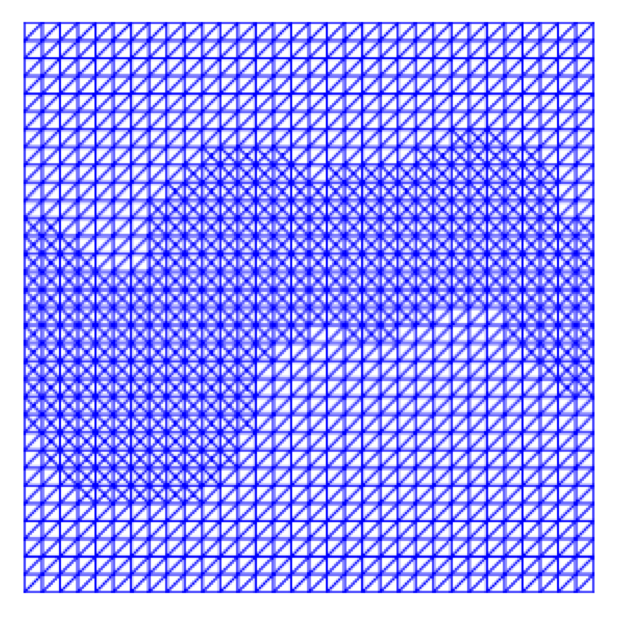
\includegraphics[width=3in]{../figures/dolfin_plot_0.png}
\caption{Unstructured mesh}
\label{fig:mesh}
\end{center}
\end{figure}


System (\ref{eq:system}) is symmetric but indefinite, and therefore the appropriate Krylov method to solve this system would be MINRES \cite{paige1975solution}. At each iteration of MINRES an AMG V-cycle is applied to
$$\begin{bmatrix}
    A & 0 \\
    0 & M
\end{bmatrix},$$
as the preconditioner. Table \ref{tab:iter2d} shows the iteration numbers and solution times for several unstructured meshes.
\begin{table}[h!]
\resizebox{1.1\textwidth}{.2\textwidth}{%
\begin{tabular}{lrrrrrrrrrr}
\hline
Total  &   V DoF &  Q DoF & $ \#$ iters &  Soln  &      $||u_e-u_h||_2 $&  V-order &              $ ||p_e-p_h||_2$ &  P-order \\
 DoF &   &   &  &   Time &      &  &                &  \\
\hline
         86    &      74 &     12 &       26 &       0.00 &  1.59e+00 &     0.00 &              1.36e+01 &     0.00 \\
        232   &     202 &     30 &       47 &       0.01 &  2.35e-01 &     2.76 &               2.84e+00 &     2.26 \\
        884    &     778 &    106 &       52 &       0.02 &  2.73e-02 &     3.11 &              5.91e-01 &     2.27 \\
       3367   &    2978 &    389 &       55 &       0.10 &  3.40e-03 &     3.00 &             1.43e-01 &     2.05 \\
      13076   &   11594 &   1482 &       57 &       0.43 &  4.27e-04 &     3.00 &           3.55e-02 &     2.01 \\
      51313  &   45554 &   5759 &       56 &       1.86 &  5.34e-05 &     3.00 &           8.91e-03 &     1.99 \\
     2034862&  180762 &  22724 &       58 &       8.79 &  6.67e-06 &     3.00 &           2.23e-03 &     2.00 \\
     8105652&  720274 &  90291 &       58 &      37.50 &  8.34e-07 &     3.00 &        5.59e-04 &     2.00 \\
     32350072 &  2875106 &  359901 &       58 &     177.84 &  1.05e-07 &     2.99 &   1.40e-04 &     2.00 \\
\hline
\end{tabular}

}
\caption{Stokes iteration and timing results ($2D$)}
\label{tab:iter2d}
\end{table}

\noindent It is clear to see from table \ref{tab:iter2d} ($2D$ results) that as the total degrees of freedom (the dimension of the matrix) increases, the number of iterations to compute the solution does not change. One can also note that the time taken to compute the solution increases roughly by a factor of $4$ (linearly with respect to the matrix size). This is also a very important property of any multigrid solver. We can also see that we get the same sort of behavior from  table \ref{tab:iter3d}, which is the $3D$ results.

\begin{table}
\centering
\begin{tabular}{rrrrr}
\hline
 Total DoF &   V DoF &  Q DoF &  $\#$ iters &  Soln Time  \\
\hline
     114    &     105 &      9 &       22 &       0.02                  \\
     477    &     447 &     30 &       56 &       0.03             \\
    2587    &    2451 &    136 &       80 &       0.28             \\
   17043   &   16251 &    792 &       77 &       3.43           \\
  124074  &  118707 &   5367 &       76 &      41.66        \\
941837 &  902619 &  39218 &       77 &     575.14  \\


\hline
\end{tabular}
\caption{Stokes iteration and timing results ($3D$)}
\label{tab:iter3d}
\end{table}

\section{Conclusion}
In this project, we have looked into AMG preconditioning with a Stokes's problem on an unstructured grid.

When looking at large systems of equations it is important to consider methods that are scalable. We started by considering a geometric approach to multigrid. Applying GMG to problems that are discretisations on structured grids can perform extremely well (see table \ref{tab:multitest}). This method relies on the fact that there is an underlying grid structure that restriction and prolongation operators can be easily defined. If however one is considering an unstructured grid then it is harder to define restriction and prolongation operators that are determined from a mesh. Therefore an algebraic way to construct these operators is generally preferable.

Looking solely at the matrix coefficients an algorithm was proposed by Ruge-St{\"u}ben in the 80's to form restriction and prolongation operators without knowledge of the underling mesh. The main part of this project was to understand and describe the process in which classic AMG was first derived. In section \ref{sec:AMG} we go through the main step in which classical AMG can be implemented.

The final part of this project looked a specific example in which AMG can be applied. The example that we looked into was solving Stokes flow on an unstructured mesh. First outlining the basic principles of preconditioning, then considered these techniques with the Stokes equations.

In conclusion, using AMG as a preconditioner can be very effective on unstructured grids.

\bibliographystyle{apalike}
\bibliography{ref}




\end{document}

